\documentclass[12pt, floatsintext, jou]{apa6}

\usepackage{amssymb}
\usepackage{graphicx}
\usepackage[outdir=./]{epstopdf}
%\DeclareGraphicsExtensions{.eps}

\usepackage{enumerate}
\usepackage{apacite}
\usepackage{listings}
\usepackage{multirow}
\usepackage{todonotes}

\newenvironment{figurehere}
	{\def\@captype{figure}}
	{}

\usepackage{lipsum}
%\pagenumbering{gobble}
%\usepackage{apacite}

\linespread{1}
\usepackage{textcomp}

\DeclareGraphicsRule{.tif}{png}{.png}{`convert #1 `dirname #1`/`basename #1 .tif`.png}
\graphicspath{{./figures/}}
 
\makeatother

\title{Why do you ask? Good questions provoke informative answers.}
\shorttitle{Q\&A}
\author{Robert X.D. Hawkins, Noah D. Goodman}
\affiliation{Stanford University} 


\abstract{What makes a question useful? What makes an answer helpful? In this paper, we formulate a family of probabilistic models of question and answer behavior that differ in the amount of pragmatic reflection attributed to speakers. We compare these models based on three different pieces of evidence: First, we explore three classic effects in psycholinguistics that show an answerer's level of informativeness varies with the inferred questioner goal. Second, we jointly test the questioner and answerer components of our model using a simple question-answer communication game. Third, we use a real-time, multi-player version of this game with a wider range of conditions, which allows us to distinguish among the questioner models. We find that sophisticated pragmatic reasoning is needed to account for some critical aspects of the data. People can use questions to provide cues to the answerer about their interest, and can select answers that are informative about inferred interests. The best model accurately fits our behavioral data, providing a promising direction for understanding the dynamics of human question-answer dialog.
}

\keywords{pragmatics, computational modeling}

\authornote{This report is based in part on work presented at the 37th Conference of the Cognitive Science Society. The first author is supported by a NSF Graduate Research Fellowship and a Stanford Graduate Fellowship. Correspondence concerning this article should be addressed to Robert X.D. Hawkins, e-mail: rxdh@stanford.edu}

\begin{document}
\maketitle
\section{Introduction}

\begin{enumerate}[(1)]
\item Scenario: Q is hungry and wants A's apple.\\Q: ``Are you gonna eat that apple?''\\ A: ``Oh, go ahead!''
\item Scenario: Q is looking for a copy of \emph{Oh, The Places You'll Go!} to give to her son at graduation.\\ Q: ``Do you know how to get to the campus bookstore?''\\ A: ``It's way on the other side of campus, but there's a shop just down the street with a better selection.''
\item Scenario: Q is at office hours and wants to learn calculus.\\ Q: ``What's wrong with my answer to \#1?''\\ A: ``Well, let me remind you how to compute a derivative...''
\end{enumerate}

In these three exchanges, Q strategically chooses an \emph{indirect question}, yet still manages to send a signal to A about her intentions. 
A, in turn, reasons beyond the overt question and provides an answer that addresses Q's true interests. 
There are many reasons why we ask indirect questions: the direct question may be impolite or embarrassing, as in (1) and (2), it may be too long or costly to fully explain, as in (2), or we may just not know enough about the topic we're interested in to articulate our interests, as in (3). 
Depending on the circumstances, an answerer can adjust their response to be over- or under-informative with respect to the direct question, or to address a different question altogether. 
This subtle interplay highlights the prevalence of social reasoning in everyday dialogue and raises two specific questions for formal models of language: What makes a question useful? And what makes an answer helpful? 

Recent work on Rational Speech Act (RSA) models \cite{FrankGoodman12_PragmaticReasoningLanguageGames, GoodmanStuhlmuller13_KnowledgeImplicature} has mathematically formalized pragmatic language understanding as a form of recursive Bayesian inference, where listeners reason about speakers who choose utterances that maximize information gained by an imagined listener.
In this paper we extend the RSA framework to address simple question-answer dialogs.
The immediate challenge in doing so is that the speaker utility in RSA is based on direct information provided by an utterance---since questions don't provide direct information\footnote{That is, the literal meaning of a question does not seem to be new information about the world, per se. Questions do, of course, end up conveying information about the speaker's knowledge, needs, and so on---it is this conveyed information that we attempt to derive below.}, we must say what utility they do have. 

We suggest, following \citeA{VanRooy03_QuestioningDecisionProblems}, that the value of a question is the extent to which it can be expected to elicit useful information later in the dialogue. 
More specifically, for the questioner, the value of a question is the expected information gained about her interests, given the set of likely answers it may provoke. 
This diverges from regular RSA in that the value of a question depends on information gained by the speaker (rather than listener), and that this information comes later in the (very short) conversation.

To fully specify this questioner we need a model of the answerer, which can serve as both the model assumed by a questioner, and as a model of answer behavior itself. We explore three, increasingly sophisticated, answerer models. The simplest answerer provides a literal answer to the question (without attempting to be informative);   
the explicit answerer attempts to be informative with respect to the surface form of the question asked (without inferring the questioner's underlying interests);  
the pragmatic answerer infers the most likely true interests of the questioner, and then informatively addresses those interests.
The latter model uses an extension of RSA to reason about the topic of conversation, as proposed by \citeA{KaoWuBergenGoodman14_NonliteralNumberWords}; it goes beyond previous work by using the explicit question as a (potentially indirect) cue to this topic. 

%% I think we need to discuss at least one previous model, to make it clear why the problem we're tackling is a problem in the first place. The rest can be in related work at the end.
% Recent formal models of question-answer pragmatics have made progress by formally specifying the questioner's goals and what it means for an answerer to be informative with respect to them. van Rooy \citeyear{VanRooy03_QuestioningDecisionProblems}, for instance, defines a goal as a utility function defining a decision problem faced by the questioner. A useful answer under this decision theoretic account is one that maximizes the expected value of the questioner's utility by reducing their uncertainty about the true state of the world. A useful question is one that allows for a sufficiently fine-grained set of answers, optimally distinguishing the worlds relevant to their decision problem. While this framework elegantly accounts for the context-dependence and relevance-maximization of question and answer behavior, it assumes that the questioner's decision problem is known \emph{a priori} by the answerer or fully determined by context. This minimizes the role of the questioner; they just establish a space of answers and then let the answerer do the rest of the work. If the answerer is so adept at using context to determine the relevant information, though, why does the questioner need to ask a question in the first place? Is it just a formality, to prompt the other for their information, or does it serve as a signal in itself, as the studies above suggest? 
%
%We claim that the questioner must reason about answerer behavior, in order to determine what question will produce the most useful answers. This raises a further issue: what kind of answerer does the questioner reason about, and is this internal model accurate? 

The rest of this paper is structured as follows. First, we review previous experimental results and formal models from the question-asking and -answering literature. We then lay out the details of our computational questioner and answer models and present a set of computational experiments demonstrating how this set of models captures four classic answerer-sensitivity effects.
%we specify a family of questioner and answerer agents, highlighting some points of divergence from previous RSA models. 
%We then formally individuate literal, explicit, and pragmatic models in this family, which represent different hypotheses about how questioners and answerers reason about their task. 
%In particular, we compare a pragmatic answerer making inferences about the questioner's goals to two simpler models: one that takes into account only that an answerer wants to be maximally informative with respect to the explicit question asked (without inferring the questioner's underlying decision problem) and one that provides a literal answer to the question (without attempting to be maximally informative).  
Because data on \emph{questioner} behavior is relatively sparse, and these classic results did not sufficiently engage the questioner component of our model, we collected data in a real-time, multi-player communication task allowing us to manipulate private goals, potential questions, and potential answers. After testing the predictions of the different models on data from a simple version of the task, we scale up this paradigm to an experiment using a wider variety of goal sets, question sets, and answer sets. We dedicate particular attention in this task to one critical condition in which the three questioner models make different predictions, allowing us to distinguish between them.
%We find that the most sophisticated, pragmatic models best account for human performance.
%derive predictions for a  of experiments using a novel guessing-game task, and compare these predictions to human performance. 
%In one phase of the task, we require participants to ask a question (from a fixed set of possible questions), given a decision problem. In the second phase, we require participants to give an answer (from a fixed set of possible answers) to a question (from a fixed set of possible questions). 
We close with a brief discussion of how our approach grounds question-asking and answering in social cognition, noting the potential scalability of our framework to problems in natural language understanding and active learning.

\subsection{Empirical background}

A number of psycholinguistic studies have provided evidence that answerers are both sensitive to a questioner's goals and attempt to be informative with respect to those goals.
For instance, in Clark's \citeyear{Clark79_IndirectSpeechActs} classic study, researchers called liquor merchants and opened the conversation with one of two sentences to set context: ``I want to buy some bourbon'' (the \emph{uninformative} condition) or ``I've got \$5 to spend'' (the \emph{five dollar} condition). They then asked, ``Does a fifth of Jim Beam cost more than \$5?'' Merchants gave a literal yes/no answer significantly more often in the latter condition than the former, where an exact price was more common. 
When provided with the five dollar context, the merchant inferred that the questioner's goal was literally to find out whether or not they could afford the whiskey, hence a simple `yes'  sufficed. 
In the uninformative context, however, the merchant inferred that the questioner's goal was just to buy whiskey, so the exact price was the most relevant response \cite{Clark79_IndirectSpeechActs}. 

Context and questioner goals have also been implicated in accounts of answers to questions like ``Do you have the time?'' that permit answers with different degrees of approximation to the true time \cite{DerHenstCarlesSperber02_RelevanceTellingTime, GibbsBryant08_OptimalRelevance}. 
To study answerer behavior, \citeA{DerHenstCarlesSperber02_RelevanceTellingTime} approached people in public places and asked for the time. Participants typically rounded their answers to the nearest 5 or 10 minute interval, even when they were wearing a digital watch. 
This showed that answerers were not simply reducing their \emph{own} effort, since rounding a time displayed on a digital watch requires an extra processing step. 
Furthermore, if the experimenter indicated that they had an appointment at a given time, they found that answers were more likely to be precise when the true time was closer to the appointment time.  
In a later study, \citeA{GibbsBryant08_OptimalRelevance} introduced a condition in which this question was preceded by the statement ``My watch stopped,'' and found that answerers were more likely to make their response precise to the minute. 
An approximate time is sufficiently informative with respect to most common goals, like making it to a meeting on time, yet answerers were able to adjust their response after inferring a less common goal, like setting a watch, which required more precise information.

Similarly, questions like ``where are you?'' permit answers at many degrees of specificity: \emph{the United States}, \emph{my apartment}, and \emph{by the big tree} are each perfectly appropriate in some context (and highly inappropriate in others). 
\citeA{Potts12_CardsDialogueCorpus} investigated the relationship between questioner goals and answerer sensitivity using the Cards corpus, a collection of transcripts and associated contextual information from a two-person collaborative game. 
In the game, two players were placed in a virtual world where they were instructed to collect cards with six consecutive numbers from the same suit. Each player could only hold three cards at a time, and neither player could see the other, thereby requiring the players to explicitly coordinate their locations. 
Using an information-theoretic measure to quantify a response's degree of specificity, Potts found that answers tended to be more specific when the questioner was trying to meet up or direct the answerer to a specific card, and less specific when developing a general search strategy. 

There are a number of other phenomena that have motivated formal pragmatic accounts of answers, but which have not been studied experimentally. 
For example, identification questions like ``who is X?'' can be resolved in many ways  \cite{BoerLycan75_KnowingWho, Gerbrandy00_Identity, Aloni05_ConceptualCovers}. 
If an undergraduate asked ``Who is Noam Chomsky?'' in an introductory course, it would be appropriate to respond ``The MIT professor who wrote \emph{Aspects of the Theory of Syntax}'' or ``The father of modern linguistics.'' If a potential donor asked the same question at an MIT fundraiser, though, it would be more appropriate to point at Chomsky in the crowd. 
Similarly, if a child asks ``What's that?'' while pointing at a common household object, a parent's response will be much different than if one of their adult friends asked the same question. More specific \emph{wh}-questions like ``Who passed the examination?'' have also been studied extensively in developing linguistic theories: answers can be understood to mean either an \emph{exhaustive} or \emph{selective} list of relevant entities \cite{SchulzVanRooij06_ExhaustiveInterpretation}.

% "WHY ARE WE DOING THIS?" paragraph
Collectively, this work suggests that \emph{social inference} is a critical aspect of question-asking and answering. Note that the vast majority of prior work on question-answer behavior has focused on the \emph{answerer}, holding the question constant and investigating the effect of different contexts. 
However, questioners must also select between many alternative questions in order to achieve their goal, and their utterance serves as a signal that prompts a relevant response from the answerer. While it is clear that the answerer uses questioner goals, it remains unclear how the answerer \emph{infers} this goal from the question utterance, and to what extent the questioner is reasoning about the answerer when choosing their question. 

\subsection{Modelling background}

\todo[inline]{ndg: need a clearer explanation of why van rooij isn't enough / why it needs to be merged into the RSA framework.}

The above probabilistic model of question and answer behavior bears some resemblance to recent decision theoretic \cite{VogelBodoiaPottsJurafsky13_GricePOMDP} and game theoretic \cite{Franke13_GameTheoryPragmatics} models of pragmatic reasoning in language use. In particular, all these approaches emphasize \emph{inference} about a partner's underlying mental state. In this respect, these theories contrast with the interactive alignment model \cite{PickeringGarrod04_BBS_Dialogue} and competing dynamical systems models of dialogue \cite<e.g.>{FusaroliTylen15_Synergy}, where coordination occurs through a low-level process of priming and adjusting to a partner's syntactic, lexical, and phonological choices. 

While there is a growing literature on dialogue models in general, far less attention has been devoted to the specifics of question and answer dynamics \emph{per se}. The primary theoretical work in this area derives from formal linguistic theories, which focused on the notion of informativeness. In Groenendijk and Stokhof's\citeyear{GroenendijkStokhof84_SemanticsOfQuestions} foundational work on question and answer semantics, asking a question induces a partition over the space of possible worlds, where each cell of the partition corresponds to a possible answer. An answer, then, consists of eliminating cells in this partition, and the most useful answers are those that eliminate all relevant alternatives to the true world. However, as van Rooy \citeyear{VanRooy03_QuestioningDecisionProblems} and others \cite{Ginzburg95_ResolvingQuestions} have pointed out, this predicts that wh-questions like ``Where can I buy an Italian newspaper?'' can only be fully resolved by exhaustively mentioning whether or not such a newspaper can be bought at each possible location. Clearly, this is not the case: a single nearby location would suffice. These theories also cannot account for contextual variation in what counts as a useful answer.

More recent theories have tried to fix these problems by introducing some consideration of the questioner's goals. \citeA{VanRooy03_QuestioningDecisionProblems}, for instance, formalizes these goals as a decision problem faced by the questioner. A useful answer under this decision theoretic account is one that maximizes the expected value of the questioner's decision problem. A useful question is one that induces a sufficiently fine-grained partition, optimally distinguishing the worlds relevant to the decision problem. While this framework elegantly accounts for the context-dependence and relevance-maximization of question and answer behavior, it assumes that the questioner's decision problem is known a priori by the answerer. \todo{ndg: check.} If this were the case, the act of asking questions would seem irrelevant: why wouldn't the answerer directly tell the questioner which action to take?

Our models are an effort to expand on this core idea in a probabilistic framework, which also provides a mechanism for the answerer to \emph{infer} the `decision problem.' 
The RSA framework has already been applied to account for diverse pragmatic phenomena including scalar implicature\cite{GoodmanStuhlmuller13_KnowledgeImplicature}, 
interpretation of context-sensitive adjectives like ``tall'' or ``cheap'' \cite{LassiterGoodman15_AdjectivalVagueness}, 
non-literal language use like hyperbole \cite{KaoWuBergenGoodman14_NonliteralNumberWords} and irony \cite{KaoGoodman15_IronyCogSci}, 
and acquisition \cite{FrankGoodman14_InferringWordMeanings}. 
Our model situates question-answer behavior within this unifying view of language understanding as recursive social inference, allowing us to formulate and evaluate competing hypotheses about what that inference entails. 


 \begin{figure*}[t]
\begin{center}
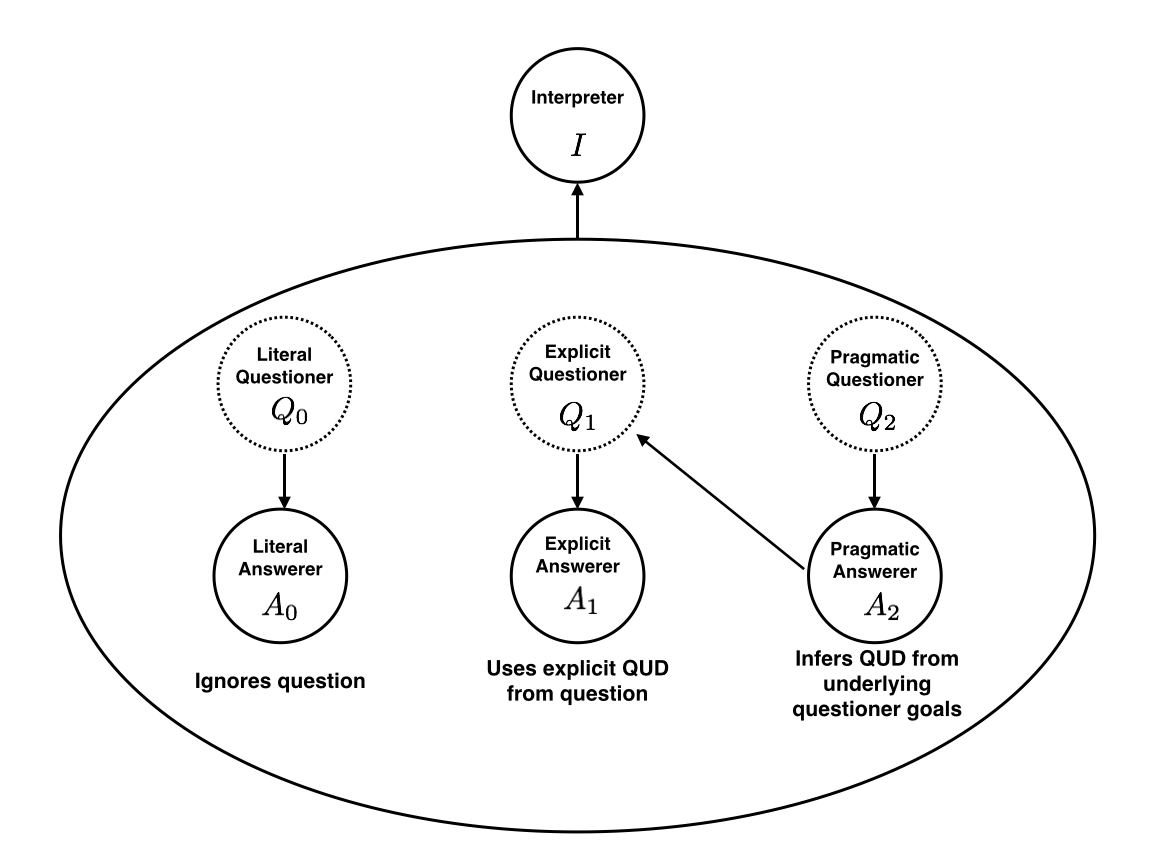
\includegraphics[scale = .75]{models.png}
\end{center}
\vspace{-.25cm}
\caption{Models.}
\label{fig:models}
\end{figure*}

\section{A Rational Speech Act model of question and answer behavior}
\label{sec:model}

\subsection{The Questioner}

How should a questioner choose between questions?
%
We start by assuming that the questioner aims to \emph{learn information relevant to a private goal}.
%
In order to choose a question that results in useful information, the questioner reasons about how the answerer would respond, given different possible states of the world; she selects a question that results in an answer that tends to provide goal-relevant information.
%

% This is a divergence from previous RSA models, where agents choose utterances with the goal of imparting information about the state of the world.

More formally, suppose there is a set of world states $\mathcal{W}$, a set of possible goals $\mathcal{G}$, a set of possible questions $\mathcal{Q}$, and a set of possible answers $\mathcal{A}$.
These sets are taken to be in common ground between the questioner and the answerer.
We formalize the notion of an informational goal $g \in \mathcal{G}$ as a projection function that maps a world state $w$ to a particular feature or set of features that the questioner cares about; this is similar to the notion of a question-under-discussion \cite<QUD;>{Roberts96_InformationStructureDiscourse}. QUDs are often used in formal linguistic models to capture \emph{relevance}: there are many informative sentences one can say to convey a world state, but only a few which are informative \emph{with respect to} the current topic of discussion.

We will denote a distribution over the set of world states by $P(w)$, and will correspondingly use the notation $\widehat{P^g}(w)$ to indicate the probability of the $g$-projection of $w$ under the projected distribution. Note that this is potentially very different from $P(g(w))$, the probability of the projected world state under the original distribution. Instead, 
$$\widehat{P^g}(v) = \int_{\mathcal{W}} \delta_{v=g(w)}P(w)dw$$ is a distribution over the image of $g$.

\todo[inline]{i also think we should add subscripts of the different model components ($Q_0$, etc). should make a figure illustrating these components....

we need to unpack and explain the math in this section more (since we have room in the long paper version).}

\newcommand{\KL}[2]{\ensuremath{D_{KL}({#1}\, \| \, {#2})}}
\newcommand{\E}[2]{\ensuremath{\mathbb{E}_{#1}\left [#2 \right]}}

The \textbf{questioner} takes a goal $g \in \mathcal{G}$ as input and returns a distribution over questions $q \in \mathcal{Q}$:
%
$$ 
\begin{array}{rrl}
P_{Q_i}(q|g) & \propto \exp \left\{ \right. & \E{P(w^*)}{\KL{\widehat{P^g}(w|q, w^*)}{\widehat{P^g}(w)}} \\[.5em]
& & \left. - \,\,C(q)\right\} 
\end{array}
$$
%\todo[inline]{ndg: hmm... i think this isn't quite right: as defined $P_g$ isn't a distribution (on W). i think what we want is the KL of the g-projections of each distribution on W. this then raises a question about whether the KLs for different goals are comparable in the right way -- e.g. smaller g-images have less capacity for information gain -- is this right?}
%
It trades off the cost of asking a question, $C(q)$, and expected information gain. The expectation is taken over all possible true worlds $w^* \in \mathcal{W}$ because the questioner has uncertainty over which true world is actually the case (represented by the world prior $P(w^*)$). The cost likely depends on question length, among other factors. Information gain is measured as the Kullback-Leibler divergence between the ($g$-projected) prior distribution, $\widehat{P^g}(w)$, and the $g$-projection of the posterior distribution one would expect after asking a question $q$ whose answer reflected true world state $w^*$:
%
$$P(w|q, w^*) = \sum_{a \in \mathcal{A}} P(w |q, a) P_{A_i}(a| q, w^*)$$
%
%This conditional distribution reflects the fact that the answerer (who knows the true world state $w$) may behave noisily, have a limited set of possible answers, or other limitations.
%to questioner (who is inferring a world state $w^*$) is affected by stochastic answerer behavior and a limited set of possible answers. 
This distribution has two components: 
First, it depends on $P_{A_i}(a | q, w^*)$, a model of likely answerer behavior which we will explore shortly. We index the questioner and answerer models by $i$ because we want to formulate different questioner models $Q_i$ which reason about different answerers $A_i$.

Second, it depends on
%\todo[inline]{ndg: I don't think we want the goal projection here. we want the distribution over worlds, in order to get a posterior distribution on worlds. . (note: need to check against implementation.)}
$P(w | q, a)$, an `interpreter' that specifies the likelihood assigned to different worlds given question and answer pairs. Note that the interpreter does not depend on goals: we will only project along $g$ in the KL operator above after we have computed the posterior.

To define the interpreter function, which all agents use to compute the literal interpretation of a question-answer pair, we must assign questions and answers a semantic meaning.
We assume that a question is an informational goal that maps from worlds to the answer set $\mathcal{A}$.
This is equivalent to the more common partition semantics of \citeA{GroenendijkStokhof84_SemanticsOfQuestions}, as can be seen by considering the pre-image of such a projection; an answer is a map from a question to a function picking out an element of the answer set given the true world: $a(q)(w)$.
\todo[inline]{rdh: Need to make this actually match the code (issue with question-answer independence)}
% \red{JD: how can we see this, exactly?} \red{RDH: we say this in the next sentence, right? $q^{-1}(a)$ gives the cell of the partition corresponding to the given aspect of interest\dots}
%An answer-value (as opposed to the answer utterance) is a possible value of the projection function (which picks out an element of the partition via $q^{-1}(a)$).
%The explicit question can be assigned a literal meaning which is a projection from worlds to answer values (this is equivalent to the common partition semantics of questions \cite{gronendijk}).
% likelihood of a world given a question and an answer.
%For the purposes of this paper, we will use Groenendijk \& Stokhof semantics \citeyear{GroenendijkStokhof84_SemanticsOfQuestions}, where a question induces a partition $\mathcal{P}_q$ over the space of possible world and each cell of this partition is an equivalence class corresponding to a different answer. An answer, then, selects a cell of this partition, denoted by $\mathcal{P}_q(a)$, which is a set.
The \textbf{interpreter} constrains the prior on worlds to the subset of its support that is consistent with the semantics of a question-answer pair\footnote{In a complete language understanding model we would also have a semantic evaluation function that maps an answer utterance to its value in $\mathcal{A}$. For clarity we assume this is a trivial mapping and suppress it.}:
%
$$P_I(w | q, a) \propto P(w) \delta_{q(w)=a}$$

\subsection{The Answerer}

How should an answerer choose between answers to a question? What should a questioner assume about the answerer when choosing a question? We next describe three different answerer models; the questioner could assume any one of them, leading to three corresponding versions of the questioner model (see .
All answerers take a question $q \in \mathcal{Q}$ and a true world state $w^* \in \mathcal{W}$ as input and return a distribution over answers $a \in \mathcal{A}$.
%
The \textbf{literal answerer} simply chooses answers by trading off prior answer probability and how well a question-answer pair conveys the true state of the world to an interpreter:
%
$$P_{A_0}(a | q,w^*) \propto P(a) P(w^* | q, a) $$
%
For a fixed question, this is equivalent to the speaker in previous RSA models. The question enters only in specifying the literal meaning of an answer (e.g. ``yes'' and ``no'' pick out different worlds in response to different questions).
%
The \textbf{explicit answerer} additionally evaluates answers with respect to how well they address the explicit question $q$. In other words, we treat $q$ itself as a projection operator on worlds, and choose answers proportionally to how well a listener with goal $q$ would guess the true state of the world $w^*$:
%
$$P_{A_1}(a | q, w^*) \propto P(a) \widehat{P^q}(w^* | q, a) $$
This implements the simplest realistic theory of answerers: they attempt to reduce the questioner's uncertainty about the aspect of the world that they were queried about.

The \textbf{pragmatic answerer} also evaluates answers with respect to how well they address the questioner's goal, but doesn't take the question's explicit meaning at face value. Instead, the pragmatic answerer reasons about which underlying goals $g$ are likely given that a question $q$ was asked, and chooses answers that have high expected informativity:
%% FIXME: restrict to truthful answers
%
$$
P_{A_2}(a | q, w^*) \propto p(a) \sum_{g \in \mathcal{G}} P(g|q) \widehat{P^g}(w^*|q, a)
$$
Reasoning backwards from questions to goals is a simple Bayesian inversion of the (explicit) questioner using a prior on goals:
$$
P(g|q) \propto P_{Q_1}(q|g)P(g)
$$
We use the explicit $i=1$ questioner model here for simplicity, but we could make $i$th order answerers that depend on the $(i-1)$th order questioner model, with $i$ arbitrarily high. For the purposes of this paper, we will only examine the simplest $(n=2)$ pragmatic answerer, and the questioner that reasons about it -- as in previous studies using RSA models, we do not find qualitative differences in the predictions of higher-order models.
%\todo[inline]{ndg: need to say here that we could depend on a sophisticated questioner model here, but we use the simplest(?) one for simplicity....}

For all of the questioner and answerer models, we can vary how strongly optimizing they are---that is, to what extent they are sampling from the distributions defined above, and to what extent they deterministically choose the most likely element. For any such distribution over utterances, we introduce an optimality parameter $\alpha$ and transform it by $ P'(x) \propto P(x)^{\alpha} $. Furthermore, we have set the answer prior in all answerer models such that outright false responses are excluded. The answerer models naturally assign very low, but non-zero probability to these options (because they are minimally informative). However, we set them to zero probability for the sake of simplicity in reporting and visualizing predictions.
%

This concludes our specification of the model space, giving a set of three answerers and three corresponding questioners that reason about them. We have implemented these models in WebPPL, a probabilistic programming language \cite{GoodmanStuhlmuller14_DIPPL}, and runnable code for all reported simulations is available online at \url{http://hawkrobe.github.io/Q\_and\_A/}. The model predictions shown throughout the rest of the paper are computed using this implementation. 

We emphasize that our models are situated firmly at the computational level \cite{Marr10_Vision} -- these models formalize hypotheses about the problem being solved by questioners and answerers in dialogue, and they make quantitative predictions about expected behavior under different assumptions. However, we do not propose that people are actively running a recursive probability calculation online every time they ask a question; further work is needed at the algorithmic and mechanistic levels to understand exactly what cognitive and neural processes give rise to the computations we predict. We now proceed to show how our model addresses four classic examples of question and answer pragmatics from the psycholinguistics literature.

\section{Four case studies}

\todo[inline]{ndg: it would be good to make this section a bit more formal. specify the model components mathematically, not only with words, and have some kind of results figures. the figures of course don't have a ton of information, but having them makes it feel more like real results. can we model the actual data from these experiments?

also, need to give more framing about what we're doing in this section and why. it's all about exploring the sensitivity of the answerer to plausible goals of the questioner, right?}

\subsection{Clark (1979), Experiment 4}
\todo[inline]{This example is redundant with the next one -- both simply make the QUD prior dependent on a context statement. Maybe we should leave this one out, since we're already using the other Clark experiment?}
First, we show that our model can provide different---sometimes over- or under-informative---answers to the same explicit question, depending on context. For this illustration, we model the whiskey-pricing study presented in the Introduction \cite{Clark79_IndirectSpeechActs}. Recall that liquor merchants were more likely to give over-informative answers (specifying exact price) to the question ``Does a fifth of Jim Beam cost more than \$5?'' in the uninformative context (``I want to buy some bourbon'') than in the five dollar context (``I've got \$5 to spend'').

Our world state is simply the whiskey's price (\$1, \$2, \dots, \$10). There are two possible goals: learning the price of whiskey and learning whether the price is greater than \$5. \todo{ndg: would the model work the same if the a priori goal set included additional threshold or interval goals? ie would the answerer rule them out based on the question asked? alternatively maybe re-cast the >5 goal as a `can i buy' goal?} The set of answers includes exact prices as well as ``yes'' and ``no'', with lower cost for ``yes'' and ``no'' than the price statements. We model the context sentence as affecting the questioner's goal prior. When the context is ``I'd like to buy some whiskey,'' we assume that the the two goals are equally likely. When it is ``I only have \$5 to spend,'' we assume that it is 9:1 in favor of learning whether the price is greater than \$5.

\subsubsection{Results} 
\todo[inline]{ndg: need to unpack these results -- this paragraph is quite cryptic.}
When the question is ``Does Jim Beam cost more than \$5?'', the correct Boolean answer is  the most probable choice (at probability $.44$ and $.49$). Critically, there is a context-dependence for answers to this question: when prefaced with ``I'd like to buy some whiskey.'', the correct exact price answer is favored more strongly (at probability $.18$) than when the context is ``I only have \$5 to spend.'' (probability $.11$). By contrast, the literal and explicit answerers (which have no natural way to account for context) do not make differential predictions in the two situations. The literal model predicts that the answerer is equally likely to say the true Boolean answer and the true numerical answer, and the explicit model predicts that the answerer will always give the true Boolean answer, since it is the explicit question being asked. This suggests that our pragmatic \emph{answerer} is consistent with human behavior in psychologically interesting situations, passing a first, qualitative, test. 

\subsection{Groenendijk and Stokhof (1984)}

For a slightly more complex example, we consider the classic puzzle of \emph{mention-some} and \emph{mention-all} readings of wh-questions  \cite{GroenendijkStokhof84_SemanticsOfQuestions,SchulzVanRooij06_ExhaustiveInterpretation}. Some questions, like ``Who is coming to dinner tonight?'' are intended to elicit an exhaustive list of the entities that are answers. For other questions, like ``Where can I find a bathroom in this building?'', a single answer would be sufficient. 

The question ``Where can one buy an Italian newspaper?'' can intuitively be ambiguous between these meanings depending on who is asking: if it is a tourist, they probably just want to know the nearest place, but if it is a businessperson trying to build a newspaper distribution network in town, they likely want the whole list. The puzzle is determining how the same question can take on different meaning in different contexts: according to our account, this happens via an inference about the questioner's underlying goal.

Our world state is an object consisting of four cafes in town. Each cafe is assigned two properties: its distance from the speaker and whether or not it sells Italian newspapers. There are two possible goals: learning the identity of the \emph{nearest} cafe selling a newspaper and learning the identity of \emph{all} cafes selling a newspaper. The set of answers includes all 16 combinations of different cafes (e.g. ``cafe 1 and cafe 3'' or ``cafe 2, cafe 3, and cafe 4''), as well as the answer ``none''. 

The prior over answer utterances is constructed as follows: there is a 10\% chance of saying ``none,'' to allow for this outcome. Otherwise, the agent selects one of the four cafes and terminates with probability .5. If the agent does not terminate, they pick another cafe from the list and continue until either terminating or running out of possible cafes. \todo{ndg: this is a slightly awkward specification of the prior. can we just make it geometric?} This naturally gives longer answers lower probability, reflecting their higher cost of utterance. We model the context sentence as affecting the questioner's goal prior: if they say ``I'm new here,'' there is a 9:1 chance that they are interested in the closest location with a newspaper; if they say ``I'm a businessperson\dots,'' there is a 9:1 chance that they are interested in all of the newspaper locations. \todo{ndg: we need to say more about where the goals and goal priors come from, so that it's clear we know this is an unsolved issue, and also clear that the model is explaining something anyhow....}
\footnote{Note that this formulation of the problem differs slightly from the one given by \citeA{GroenendijkStokhof84_SemanticsOfQuestions}, although they easily map onto one another. In the original formulation, the \emph{answer} is fixed and the \emph{meaning} of the answer must be inferred to either be mention-some or mention-all. In our formulation, the meaning of each answer is unique and fixed, but the answerer must choose among a set of different possible answers. The same inferential machinery that our questioner uses to reason about which answer utterance the answerer will give could also be used to reason about which \emph{meaning} the answerer intends by their fixed utterance. The only difference is that the questioner would have uncertainty over a set of possible meanings instead of uncertainty over a set of possible answer utterances. We chose the latter because it more closely resembles the other scenarios we are modeling.}

\subsubsection{Results}

For concreteness, we set the world to be the following :

\begin{lstlisting}
world = {'cafe1' : [3, false],
         'cafe2' : [1, true],
         'cafe3' : [3, true],
         'cafe4' : [3, true]}
\end{lstlisting}
and enumerated over all model executions for both contexts. We find that the highest probability response given the ``I'm new here'' context is the single location ``cafe2,'' with probability 0.56. Given the ``I'm a businessperson\dots'' context, however, the highest probability response is the conjunction ``cafe2 and cafe3 and cafe4,'' with probability 0.82. Note that cafe 1 was not assigned any probability in either context because it did not sell Italian newspapers (demonstrating that the pragmatic answerer will not lie), and that the nearest cafe was given precedence in the ``tourist'' context. 

The literal and explicit answerers, as in the Clark scenario, do not have the means of making inferences about the questioner's underlying goals. Thus, both models incorrectly predicted that the context would not affect the preferred response. The literal answerer predicted that all combinations of cafes 2, 3, and 4 would be given in proportion to their prior likelihood (with no special preference given to the closest one). The explicit answerer predicted that cafe2 would be preferred in all contexts.     Crucially, the only difference between our model of this scenario and the Clark scenario is the set of QUDs, the structure of the world, and the meanings of the answers. The questioner and answerer functions stayed exactly the same.

\subsection{Gibbs Jr. \& Bryant (2008): Experiment 3}

It has been shown in previous work that people typically round their answers to the nearest 5 or 10 minute interval when asked `Do you have the time?'', even when they're wearing a digital watch \cite{DerHenstCarlesSperber02_RelevanceTellingTime}.  \citeA{GibbsBryant08_OptimalRelevance} replicated this result, and then performed a follow-up study where they preceded their question by the context ``I have a meeting at 4:00.'' They found that the tendency to round times decreased as a function of the time remaining until the stated deadline: when people were asked at 3:40, they would say ``It's 3:45,'' but when people were asked at 3:53, they would make their response precise to the minute. They explain this result by appealing to the questioner's goals: while an approximate time is sufficiently informative with respect to most goals, a questioner who is running late to an appointment may have the goal of judging whether to rush, in which case a precise time is needed. 

We take the world state to be the true current time. Unlike in the previous two scenarios, where there are only two QUDs \todo{ndg: first use of QUD?} and two contexts that make each QUD more or less likely, we now let there be a \emph{family of QUDs} and a fixed context stating the time of the appointment. This family of QUDs is parameterized by a threshold time, below which times are rounded to the nearest 5 minute increment and above which times are given exactly. For example, the QUD with the threshold set at 3:50 corresponds to a goal of wanting to learn the true time if it is higher than 3:50 and only caring about the approximate time below 3:50. The prior over thresholds ($\tau =$ 3:30, 3:35, \dots, 3:55), given a context sentence, weights each threshold by its distance to the appointment time, reflecting the intuition that the questioner will be more interested in the exact time as it approaches the appointment time.
\todo[inline]{ndg: why this set of goals? maybe derive more explicitly from assumptions about planning and travel time??}

 The set of answers is the set of times that could be given (e.g. 3:30, 3:31, \dots, 4:00), with uniform probability. Critically, the meaning of an answer is not exact: it introduces a factor in the ``interpreter'' component of the model, upweighting world states that are close to the answer utterance. In other words, we specify an ``approximate'' semantics for number references, which is necessary for rounded answers to be produced in the first place.
 \todo[inline]{need to be more careful and formal in defining the number word meanings here.
 
 in fig 1, 3:36 is just as likely as 3:34... that seems problematic.}
 
 
 
 \subsubsection{Results}
 
 To test the behavior of this model, we compare two simulations. In both, the context is ``I have an appointment at 4:00.'' In the first, the true world state is 3:34 (the `appointment far' condition); in the second, the true world state is 3:54 (the `appointment near' condition). Gibbs Jr. and Bryant \citeyear{GibbsBryant08_OptimalRelevance} found that the answerer is most likely to round to 3:35 in the `appointment far' condition, but most likely to give the exact time, 3:54, in the `appointment near' condition. Indeed, in the `appointment far' condition, the pragmatic questioner model, which infers which threshold is likely given the context and threshold, replies the rounded time `3:35' with probability 0.40 compared to the true time `3:34' with probability 0.27. In the `appointment near' condition, this pattern reverses: the pragmatic questioner model replies the rounded time `3:55' with probability 0.16 and the exact time `3:54' with probability 0.68 (see Figure \ref{fig:timeExperimentResults}).
 
 \begin{figure}
\begin{center}
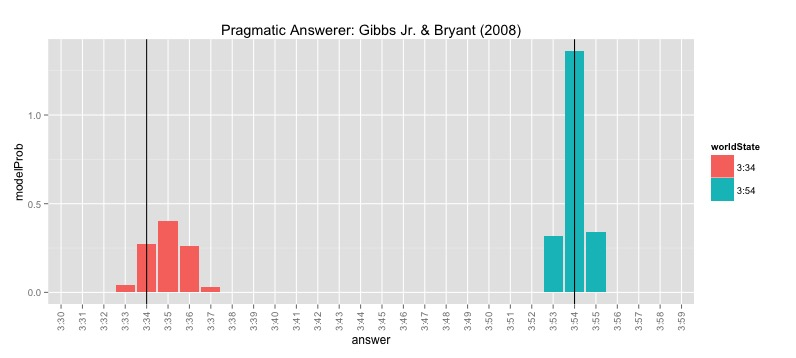
\includegraphics[scale = .5]{timeExpResults.jpeg}
\end{center}
\vspace{-.25cm}
\caption{Results for our computational experiments replicating Gibbs Jr. and Bryant (2008). Vertical lines represent the true world state.}
\label{fig:timeExperimentResults}
\end{figure}


\subsection{Clark (1979): Experiment 5}
Our final scenario is a critical test for the questioner component of our model. Because the question space in the previous computational experiments only contained one element, the pragmatic answerers' inferences were entirely based on the context and the QUD prior. One of the most interesting and novel predictions of the RSA model, however, is that the questioner's choice of utterance itself should guide a pragmatic answerer's inferences about likely underlying goals. While there are few experimental results using questioner behavior as the \emph{dependent variable}, making it difficult to test our model's predictions about questioner behavior, there is some work using the question asked as an \emph{independent variable} and testing how it affects answers.

One such study was conducted as a follow-up to the first experiment we modeled in this paper. Instead of calling liquor merchants, \citeA{Clark79_IndirectSpeechActs} called restaurants and asked one of four yes/no questions about which \emph{credit cards} the restaurant accepted:

\begin{enumerate}
\item ``Do you accept Master Charge cards?'' 
\item ``Do you accept American Express cards?''
\item ``Do you accept credit cards?'' 
\item ``Do you accept any kinds of credit cards?'' 
\end{enumerate}

He analyzed the likelihood that the respondent gave a yes/no answer, compared to the likelihood of giving the full (over-informative) list of exactly which cards were accepted.  He found that (1) and (2) were nearly always answered with a `yes' or `no', (3) was equally likely to be answered with yes/no and full information, and (4) was nearly always answered with full information. 

We formalize this scenario in our model in the following way. The set of possible worlds is given by an object mapping five differents kinds of cards (`Visa', `MasterCard', `American Express', `Diner's Club', and `Carte Blanche') to a Boolean representing whether or not they are accepted. The true world state is known by the answerer but not the questioner. The above four questions form the question space, and the answer space contains `yes', `no', and all possible combinations of cards, including the empty list.

There are four possible goals, which we can understand through four possible questioner situations. First suppose that the questioner only has MasterCard. Thus, a full list would not be helpful -- they only want to know whether or not MasterCard is accepted. This is the ``MasterCard'' goal. Second, suppose that the questioner has both MasterCard and Diner's Club. Then they want to know whether the restaurant takes \emph{either} card. This is the ``Master + Diner's'' goal. Third, suppose that the questioner has MasterCard, Diner's Club, and American Express. Then they just need to find out whether any one of these cards is accepted. This is the ``Master + Diner's + American'' goal. Finally, they might be interested in learning the actual set of names of cards accepted by the restaurant. This is the ``names'' goal. 

% learning whether or not the establishment accepts (1) Visa, (2) Discover, (3) MasterCard, or (4) learning the exact list of cards that the establishment accepts. The set of answers includes ``yes,'' ``no,'' and all possible lists of the three cards listed above, with ``yes'' and ``no'' slightly preferred for their lower cost. Because there is now a decision between different questions that the questioner must entertain, we must also specify a \emph{questioner} prior, which we set to uniform for simplicity. 

\subsubsection{Results}
  \begin{figure}[t!]
  \begin{center}
\includegraphics[scale = .7]{creditCardPlot.jpeg}
\end{center}
\vspace{-.25cm}
\caption{Results for our computational experiments replicating Clark (1979), Experiment 4. M stands for the ``MasterCard'' answer, D stands for the ``Diner's Club'' answer, and $M+D$ stands for the answer mentioning both. Note that we give an over-informative answer to ``Do you accept any kinds of credit card?'' in the left panel, but a literal `yes'/`no' answer to ``Do you accept MasterCard?'' in the right panel.}
\label{fig:creditCardExperimentResults}
\end{figure}


We tested the behavior of our pragmatic answerer on the following world state:

\begin{lstlisting}
var world = {
      'Visa' : false,
      'MasterCard' : true,
      'AmericanExpress' : false,
      'Diners' : true,
      'CarteBlanche' : false
  };
\end{lstlisting}

We find that when the questioner asks ``Do you accept MasterCard?'', the pragmatic answerer is most likely to respond `yes,' but when the questioner asks ``Do you accept any kinds of credit card?'', they are most likely to respond with the full list of credit cards accepted (see Fig. \ref{fig:creditCardExperimentResults}). 

When we examine the inferred QUD in each case, these results become clearer. For the ``MasterCard'' question, the pragmatic answerer reasons that the most likely goal is to specifically find out about MasterCard, so ``yes'' is a sufficient response. For the ``any kinds'' question, however, the pragmatic answerer reasons that the most likely goal is to get the full list of names. ``Yes'' would not adequately address this underlying goal, so the answerer chooses to give the full list instead. Note that these inferences are made purely on the basis of the questioner model's behavior rather than general context as in the previous simulations.

\todo[inline]{I'd like to extend this example a step further by having the restaurant-owner reason about \emph{which cards the caller owns}, with the assumption that asking about a larger set of cards requires the questioner to pay a higher cost (thus the ``any cards'' question). Having a possible goal be ``learning the full set'' seems a bit of a stretch.}
\subsection{Discussion}

The same questioner and answerer model reproduced patterns of question-answer behavior in four different scenarios. It captured both explicit and implicit context effects as well as effects where the question itself served as a signal about the relevant underlying goals. 
%Note that all of these studies were focused primarily on answerer behavior, allowing us to show that our model of the questioner is consistently used as an submodule of the answerer. However, because questioner behavior was always manipulated as an independent variable, we could not test the questioner model as a stand-alone predictor of human questioning behavior. This reflects a general neglect of questioner behavior in the psycholinguistics literature, and further experiments are needed to test its predictions. 
There remain some deep questions about the behavior of our model in these scenarios, particularly the final one. Recall that Clark found a difference between ``Do you accept any kinds of credit cards?'' and ``Do you accept credit cards?'' Our model treats these two questions as equivalent (with the literal semantics returning true if any of the Booleans in the object are true and false otherwise), which propagates all the way up to the pragmatic answerer. It is not obvious where the asymmetry arises. \todo{ndg: did you try just making cost different for the two?} Another issue is that our resulting answer distribution does not appear to be robust to all parameter settings and worlds. The answer prior uses a parameter to determine the likelihood of `yes' and `no' responses versus lists of card types, and different settings of this parameter yield very different absolute answer distributions (although they all appear to shift toward fewer `yes'/`no' answers and more list answers in response to the ``any kinds'' question). It will be valuable to conduct a more rigorous exploration of the model space, and also test sensitivity to QUD alternatives. 

While the questioner component of our model was critical to the pragmatic answerer's behavior in the final simulation, none of these scenarios truly tested the questioner component.  Indeed, most empirical work has treated the question or context as an independent variable, with the answer as a dependent variable. Our model, following \citeA{VanRooy03_QuestioningDecisionProblems}, however, suggests that the question itself is important in prompting a relevant answer. In order to test these predictions, we designed a sequence of experiments using a communication game to collect data on both question-asking behavior \emph{and} question-answering behavior.

\todo[inline]{ndg: random note about politeness: we often use more words than necessary, just to avoid seeming curt. for instance i'd bet a lot of the 'yes' answers in the credit cards experiment are actually something like 'yes, we do'. one way to think about this is that the answerers relative balance between cost and helpfulness (roughly how much they care) is unknown to the questioner, and questioners will infer this. thus the answerer will choose answers partly to signal that they value helping.}

\section{Exp.~1: Interactive Questions and Answers}

\subsubsection{Participants} We recruited 50 participants
from Amazon's Mechanical Turk to participate in this task: 25 were assigned to the  questioner role and 25 to the answerer role, yielding 25 complete games.

\subsubsection{Stimuli \& Procedure} The world space $\mathcal{W},$ goal space $\mathcal{G}$, question space $\mathcal{Q}$, and answer space $\mathcal{A}$ were the same as in experiment 1 (see Figure \ref{fig:taskhierarchy}). The procedure was modified to accommodate real-time player-to-player interaction following \citeA{Hawkins14_RealTimeWebExperiments}. All players passed a short quiz on the game instructions and were immediately redirected to the game interface: the first player to join was assigned to be a ``questioner'' (which we called a ``guesser'' in the cover story) and told to wait until a second player was available. Once another player joined, they were assigned to be an ``answerer'' (or ``helper'') and the game began. 

	\begin{figure}[t!]
\begin{center}
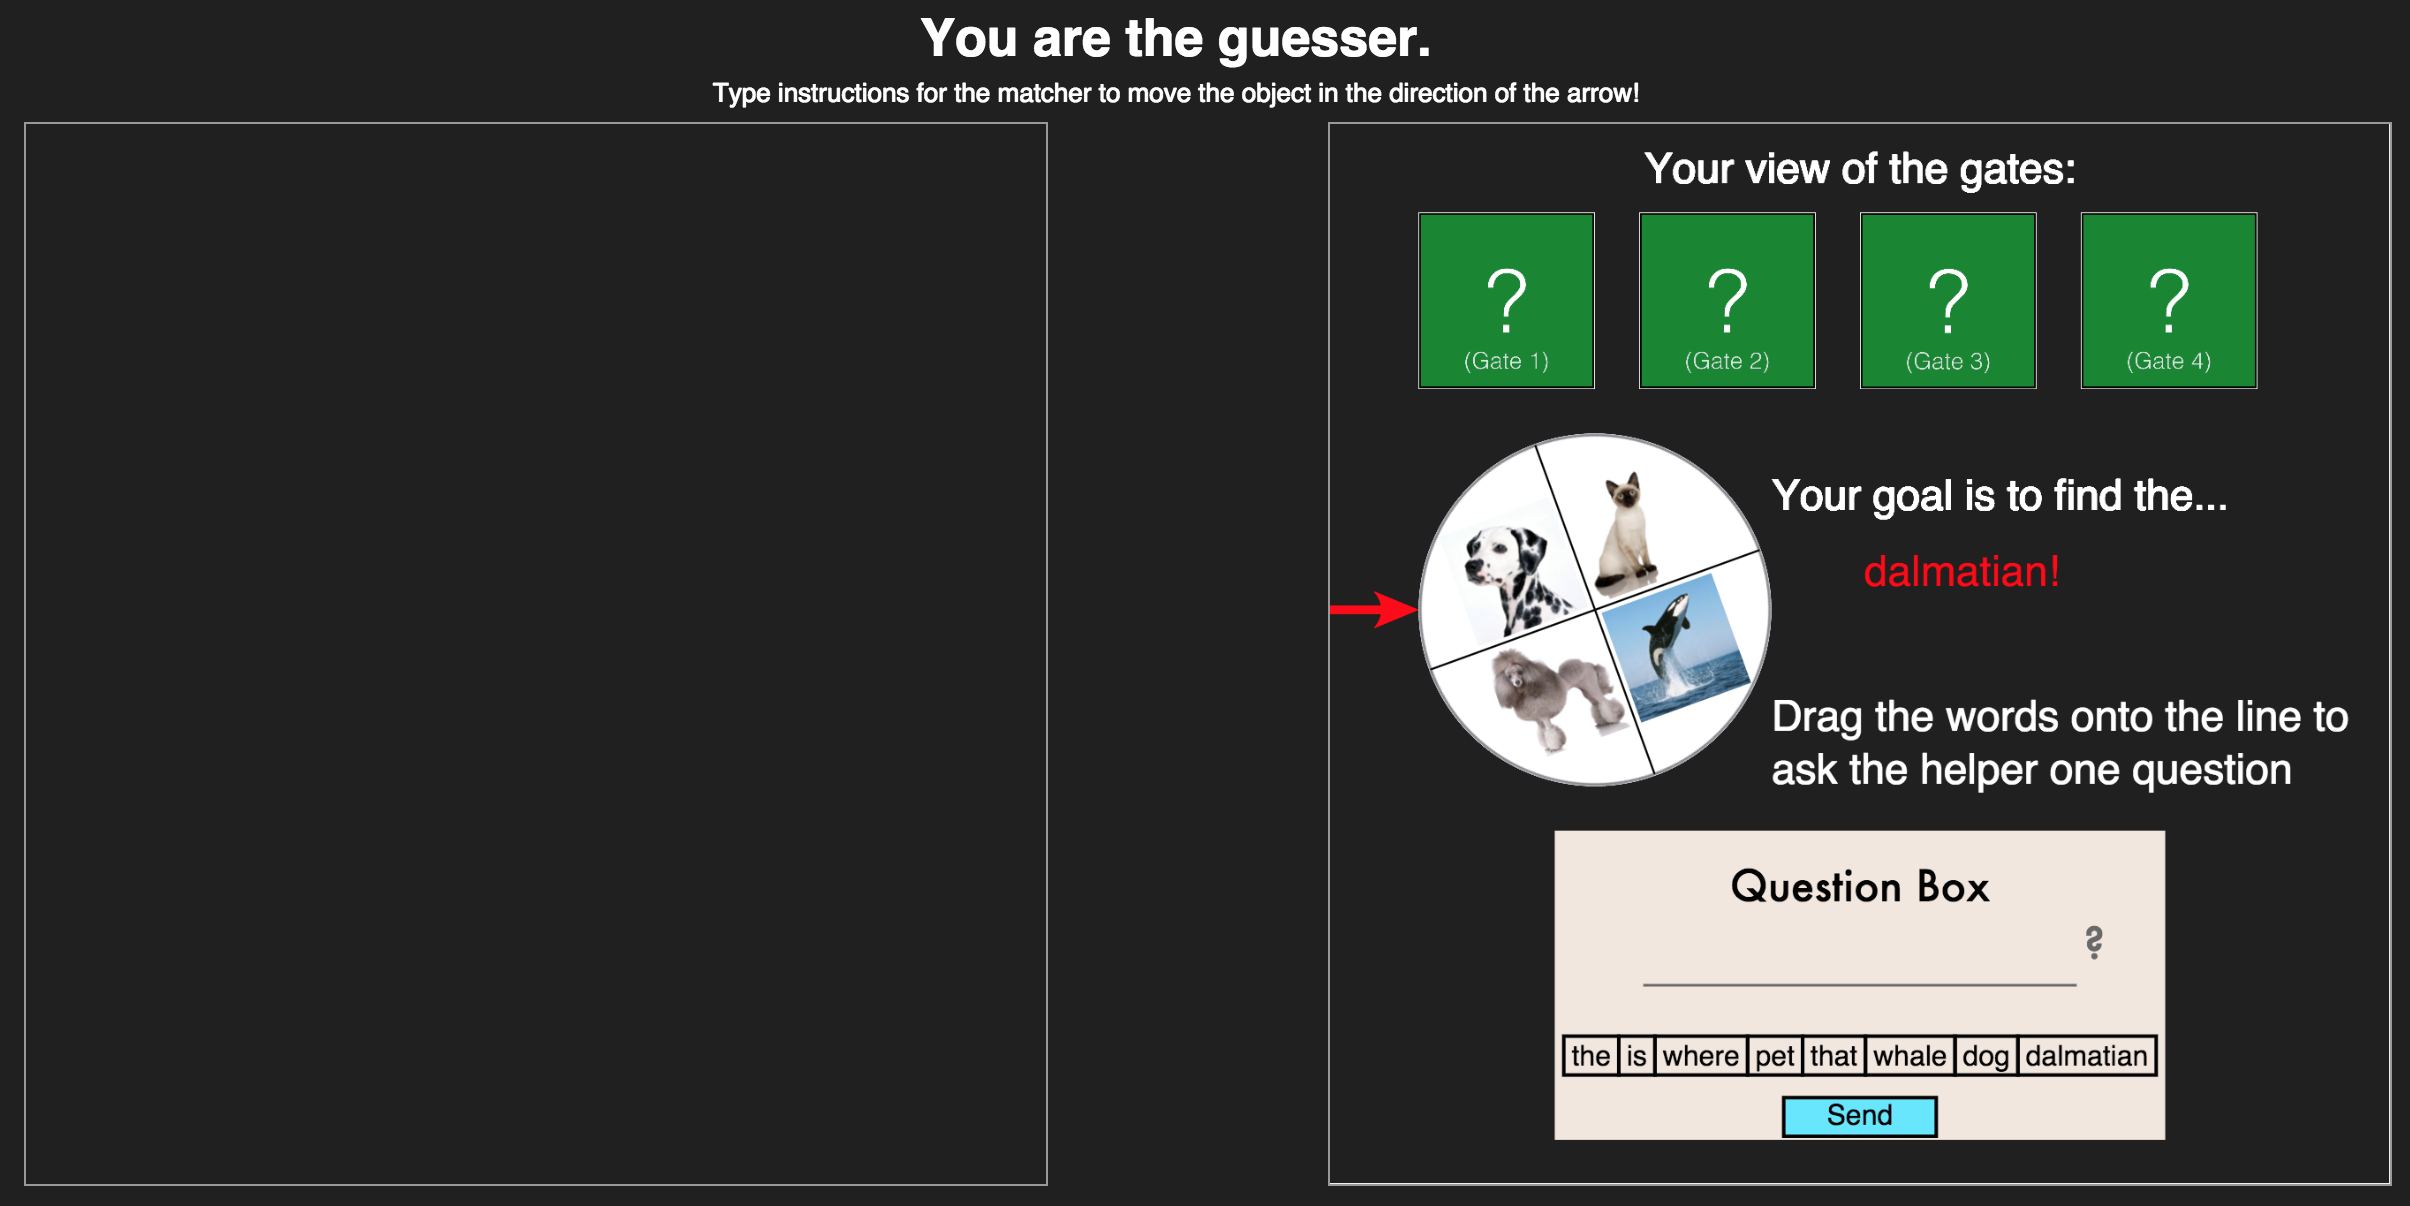
\includegraphics[scale = .3]{Exp3GuesserView}
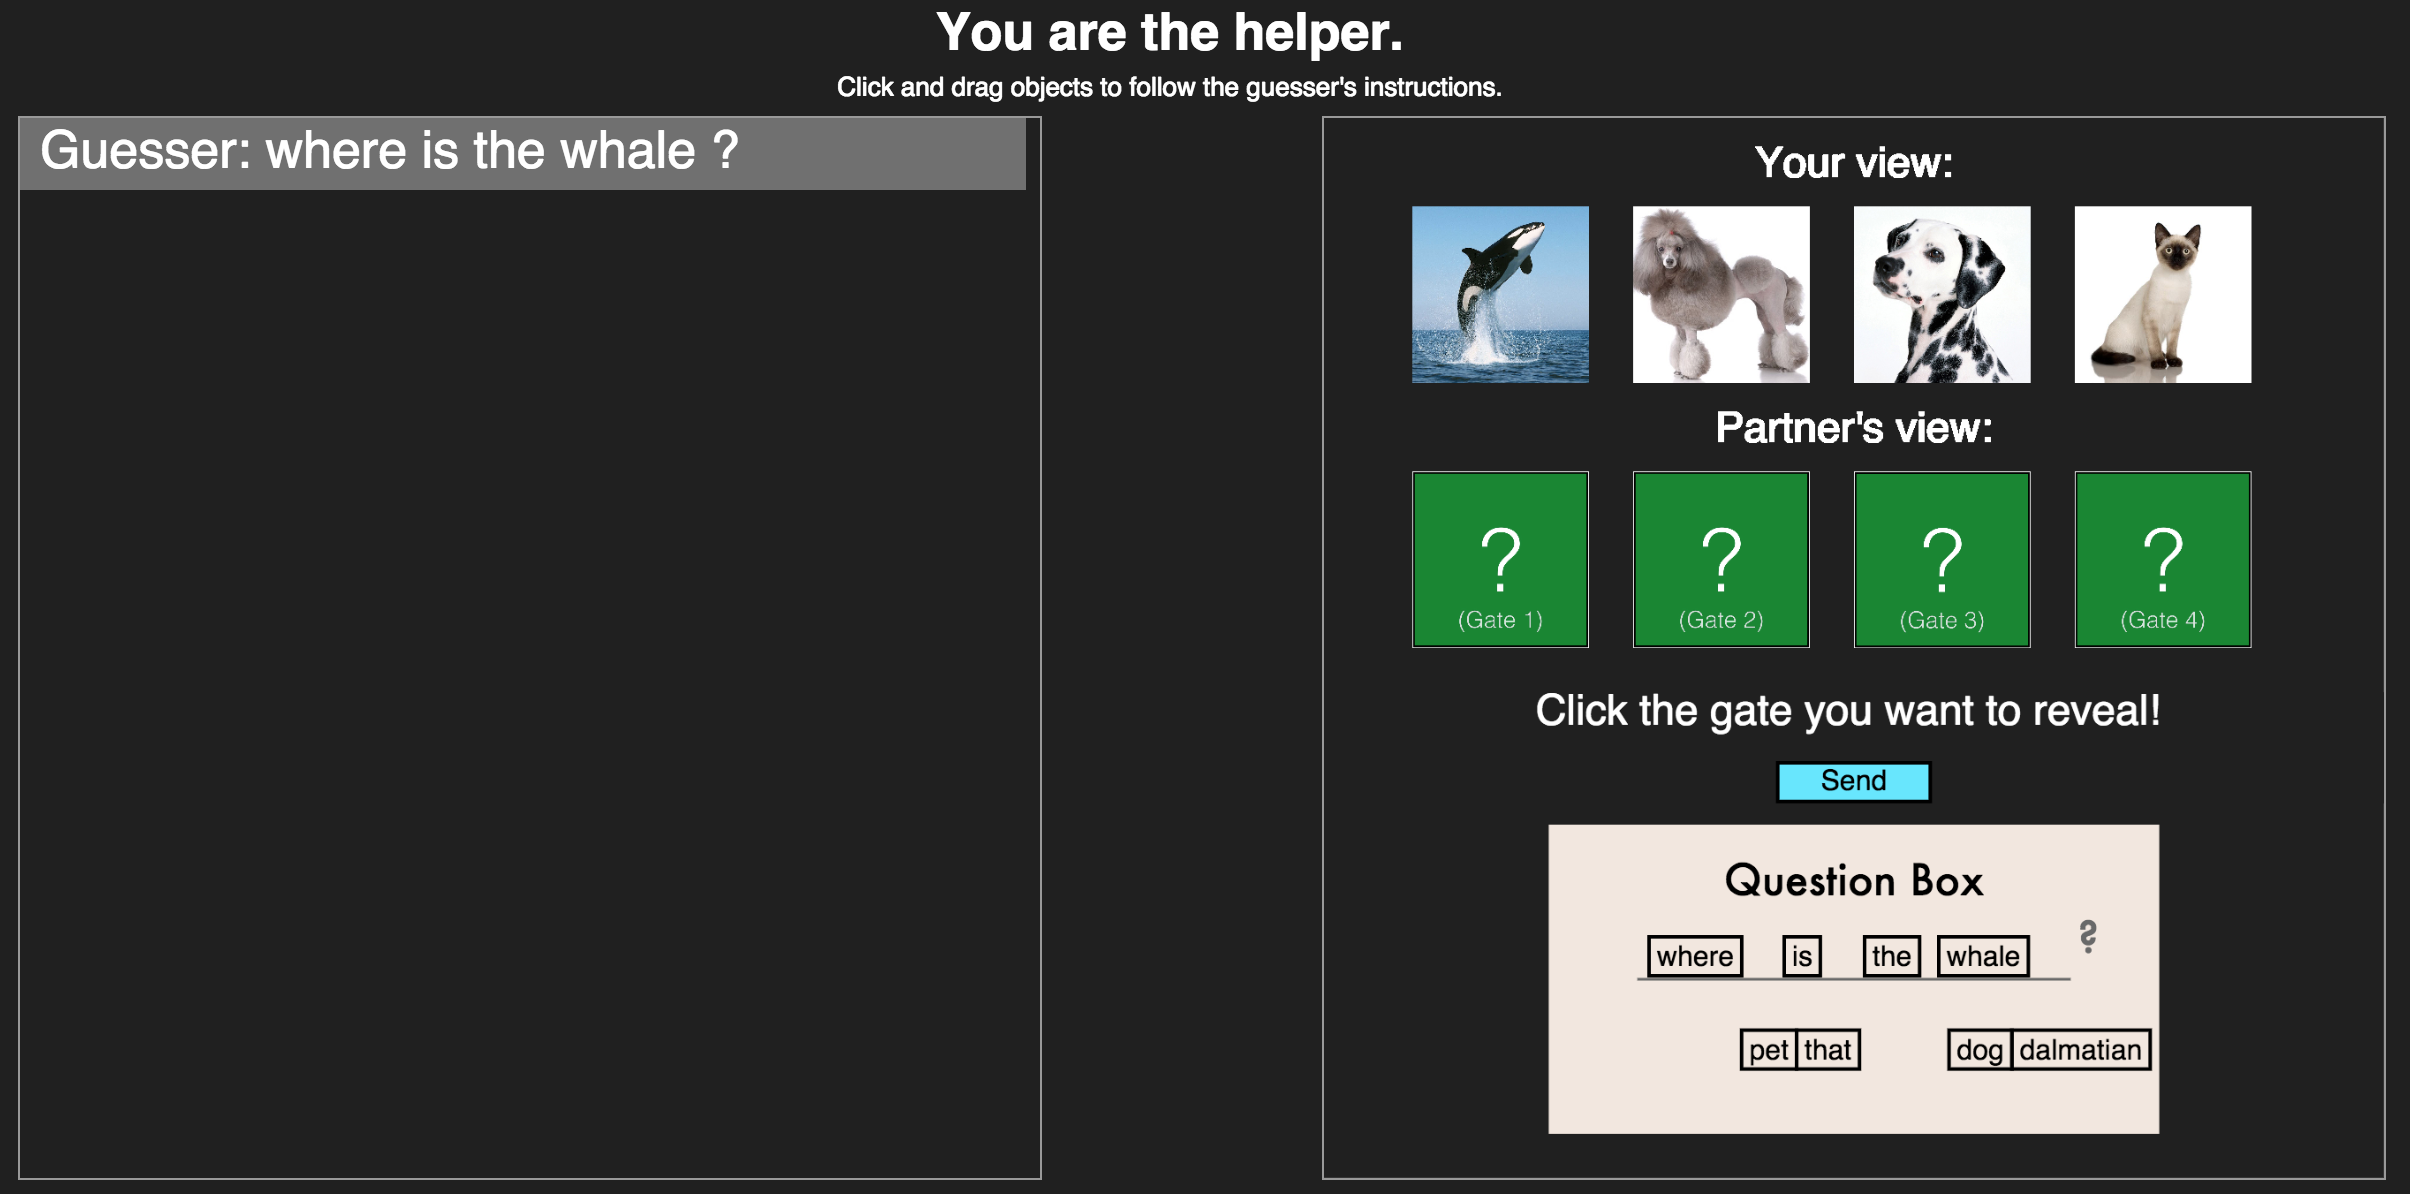
\includegraphics[scale = .3]{Exp3HelperView}
\end{center}
\vspace{-.5cm}
\caption{Exp.~3 interfaces, for the questioner (top) and answerer (bottom).}
\vspace{-.1cm}
\label{fig:exp3views}
\end{figure}

The questioner and answerer interfaces are displayed in Figure \ref{fig:exp3views}. Chat messages were printed on the left side of the screen, and players used the right side as a workspace to view goals, ask questions, and respond with answers. At the beginning of each trial, the wheel on the questioner's screen (Figure \ref{fig:exp3views}, top) would spin and select one of the four goals. The questioner then clicked and dragged words onto the line in the ``Question box'' to ask a question to help them find this goal. The answerer saw these words being dragged in real time. Once the questioner clicked the `send' button, the resulting question appeared in the chat log and control was passed to the answerer, who clicked on one of the four gates to send a response containing the location of the chosen object. Finally, the questioner was asked to guess which gate they believed the goal object was behind. 

Each participant provided responses for four trials, where object locations were shuffled and a new goal was randomly selected for each trial. Thus, questioners could be given the same goal on multiple trials, preventing `process of elimination' reasoning about what the goal may be on the part of the answerer. 

\subsubsection{Results}
%\red{check for effect of Q/A block order.}
Results for the questioner role are shown alongside model predictions in Fig.~\ref{fig:exp3res} (left). We find that questioners systematically prefer to ask different questions given different goals, even as those questions become more indirect. $\chi^2$ tests over each of the four response distributions show a significant divergence from uniform. Questioners preferentially ask about the `dalmatian' given the  dalmatian goal, ${\chi^2(3) = 77}, {p < .001}$, about the `dog' given the poodle goal, ${\chi^2(3) = 50}, {p <.001}$, about the `pet' given the cat goal, ${\chi^2(3) = 47},  {p <.001}$, and about the `animal' when given the whale goal, ${\chi^2(3) = 39}, {p <.001}$. Note that there was a high level of agreement between participants: responses were not particularly graded.

Results for the answerer role are shown in Fig.~\ref{fig:exp3res} (right). Answerers are highly sensitive to the constraints of the questioner, giving information about the dalmatian when asked about a `dalmatian', ${\chi^2(3) = 102}, {p <.001}$, about the poodle when asked about a `dog', ${\chi^2(3) = 47}, {p <.001}$, about the cat when asked about a `pet', ${\chi^2(3) = 45}, {p<.001}$, and about the whale when asked about an `animal', ${\chi^2(3) = 31}, {p < .001}$. In the next section, we compare these results to the predictions of our family of models (Fig. \ref{fig:Exp3ModelSpace}). 

\begin{figure}[t!]
\begin{center}
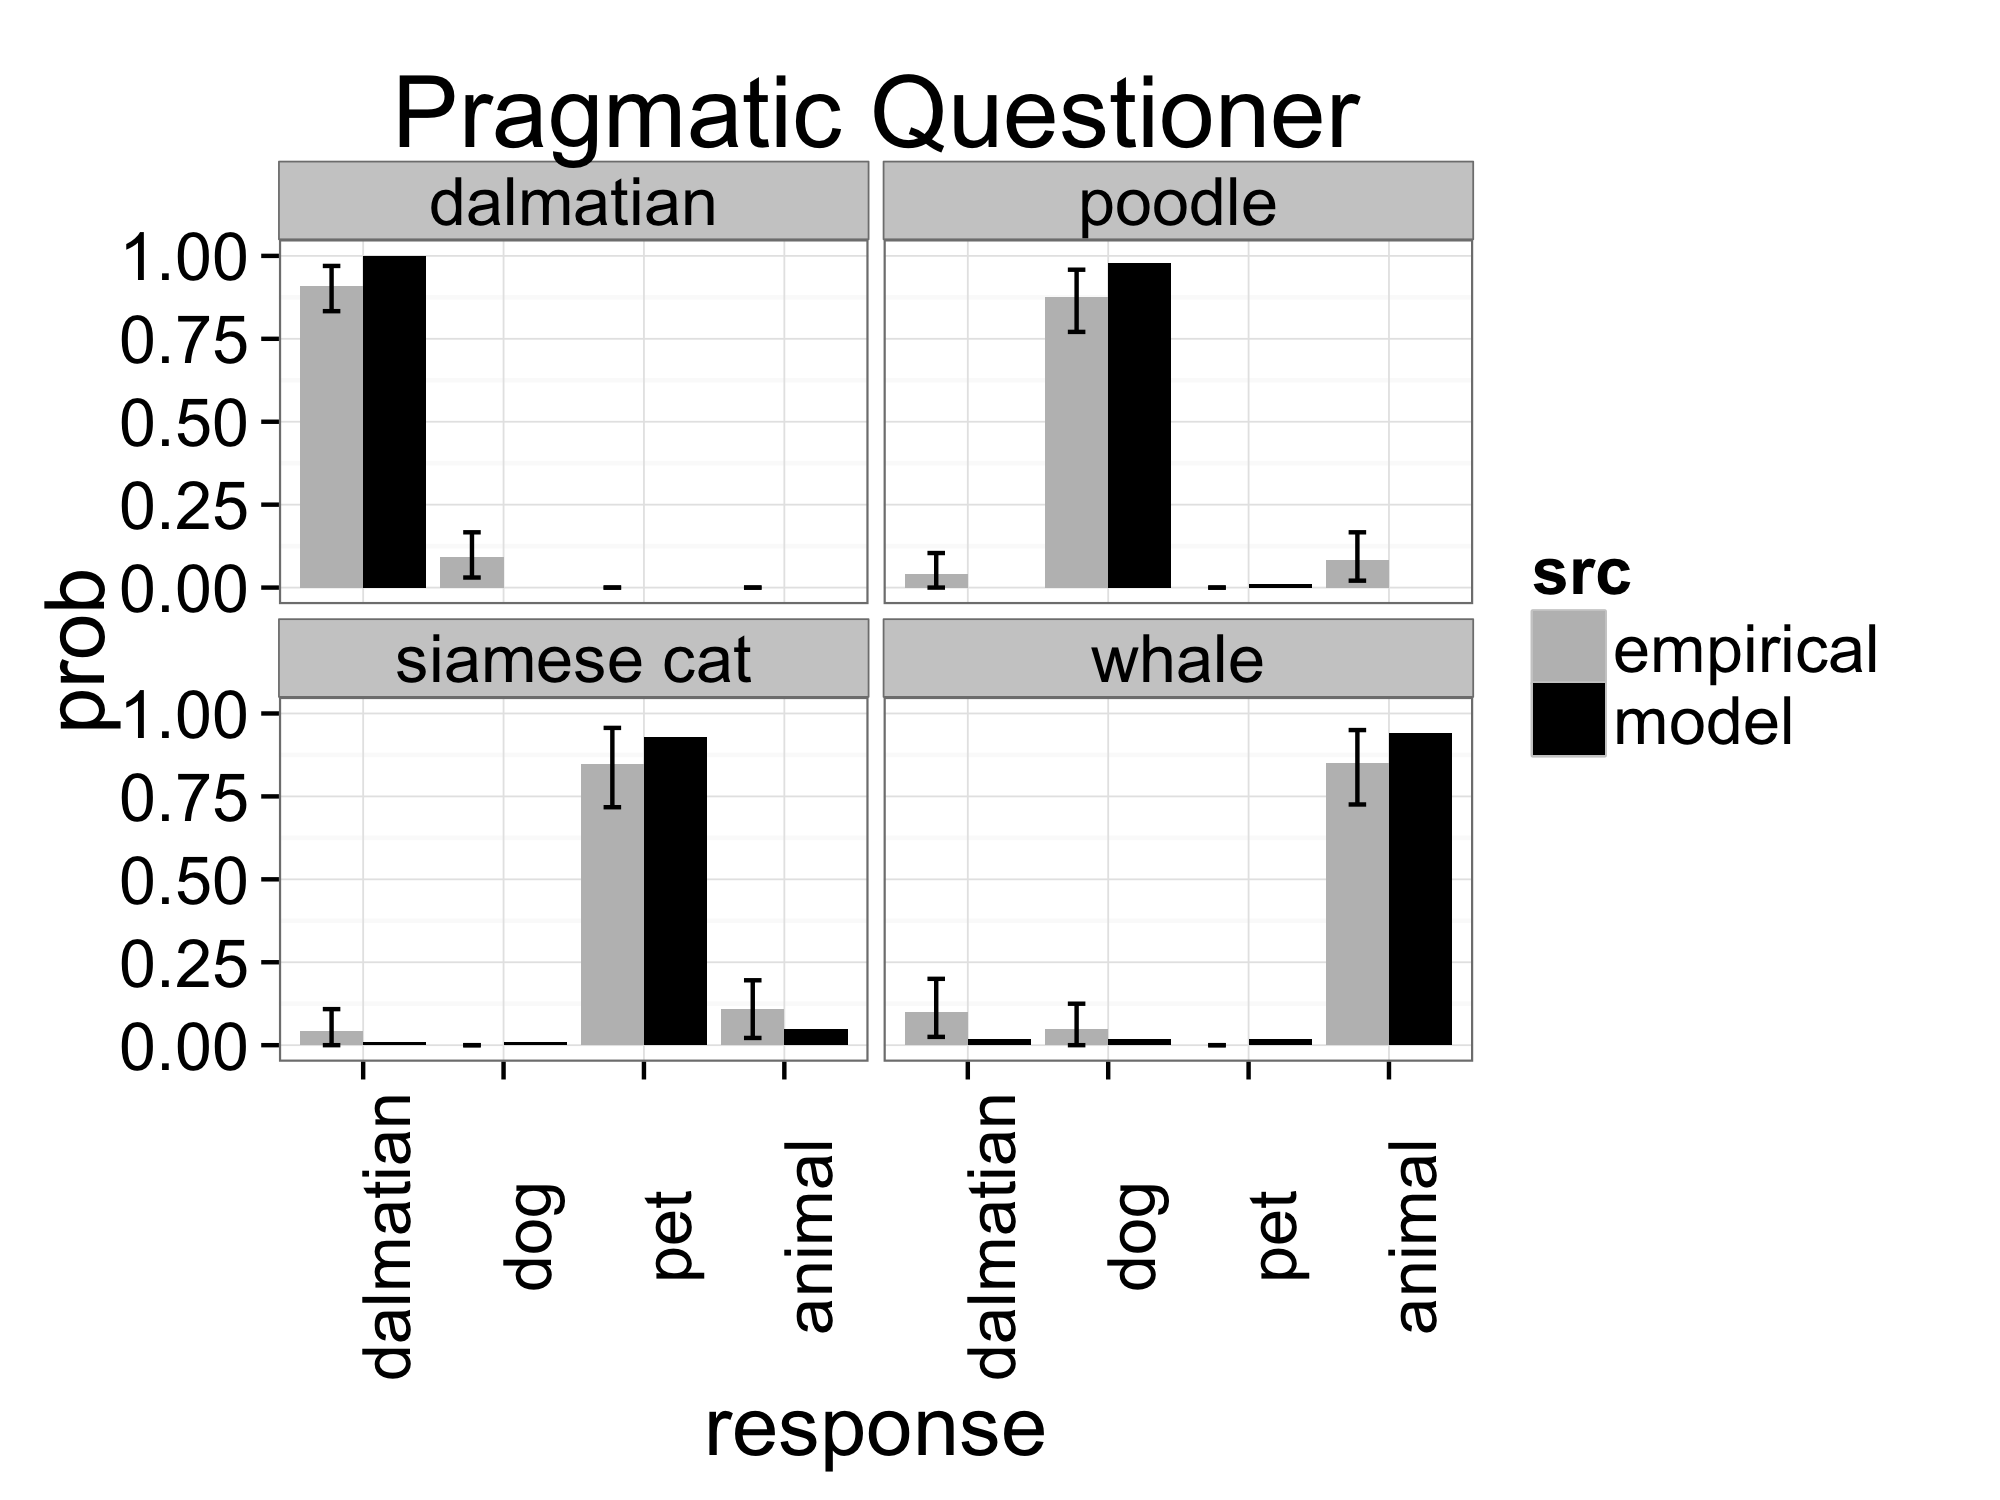
\includegraphics[scale = .11]{exp3QuestResultsPragmatic.png}
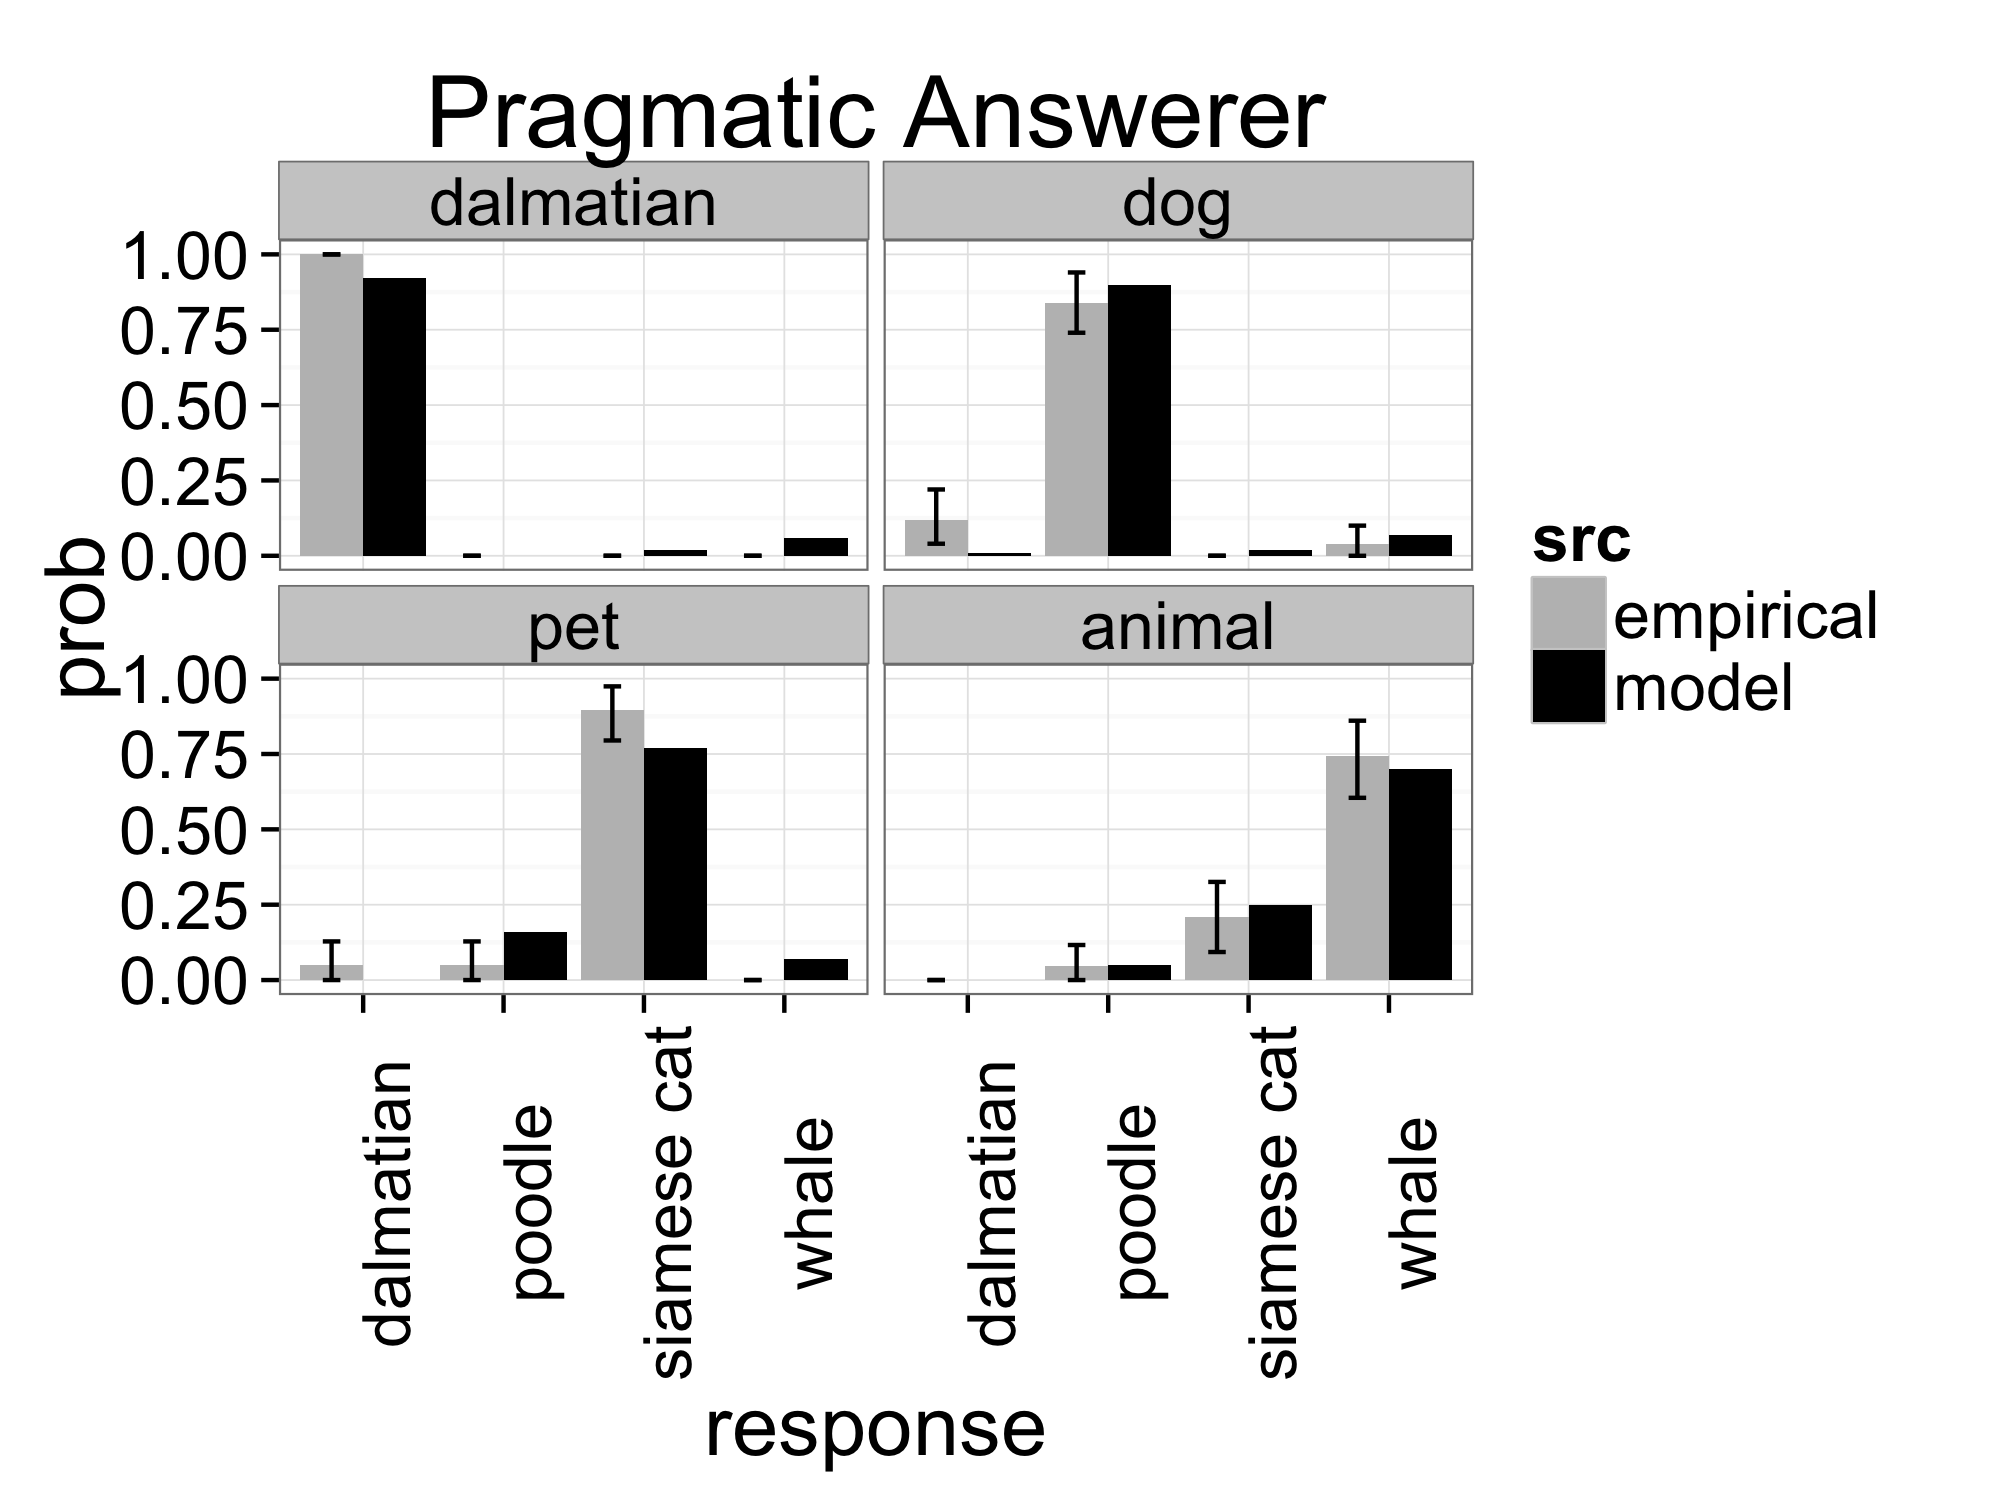
\includegraphics[scale = .11]{exp3AnsResultsPragmatic.png}
\end{center}
\vspace{-.5cm}
\caption{Exp.~3 results and model fits, for the best-performing questioner (left) and answerer (right) models. Error bars are 95\% bootstrapped confidence intervals.}
\vspace{-.1cm}
\label{fig:exp3res}
\end{figure}

\subsubsection{Model comparison}

Model comparison was conducted in the same way as in Experiment 1: a single optimality parameter, which applied to all agents, was fit for each of the six models to maximize correlation with the data.

We can again rule out both the literal answerer and literal questioner as they predict a uniform distribution of responses over the four questions and answers. The two remaining questioner models again make roughly the same predictions for this task:
we found a model-data correlation of $r = 0.971$ for the explicit questioner and correlation of $r = 0.996$ for the pragmatic questioner. The difference between these correlations is statistically significant, accounting for their shared dependence on the empirical data (Zou's confidence interval $= [-0.079, -0.009]$). However, they make nearly identical qualitative predictions; the pragmatic questioner model's predictions for each response distribution are shown in Fig.~\ref{fig:exp3res} (left). 

The pragmatic answerer provides a much better fit to the data than the explicit answerer: we find a model-data correlation of $r = 0.7$ for the explicit answerer and $r = 0.99$ for the pragmatic answerer.  Taking into account the fact that these correlations are dependent and overlapping on the same empirical data, we find that the pragmatic answerer correlation is significantly larger than the explicit answerer correlation (Zou's confidence interval $= [-0.676, -0.107]$). 
%
\begin{figure}[t!]
\begin{center}
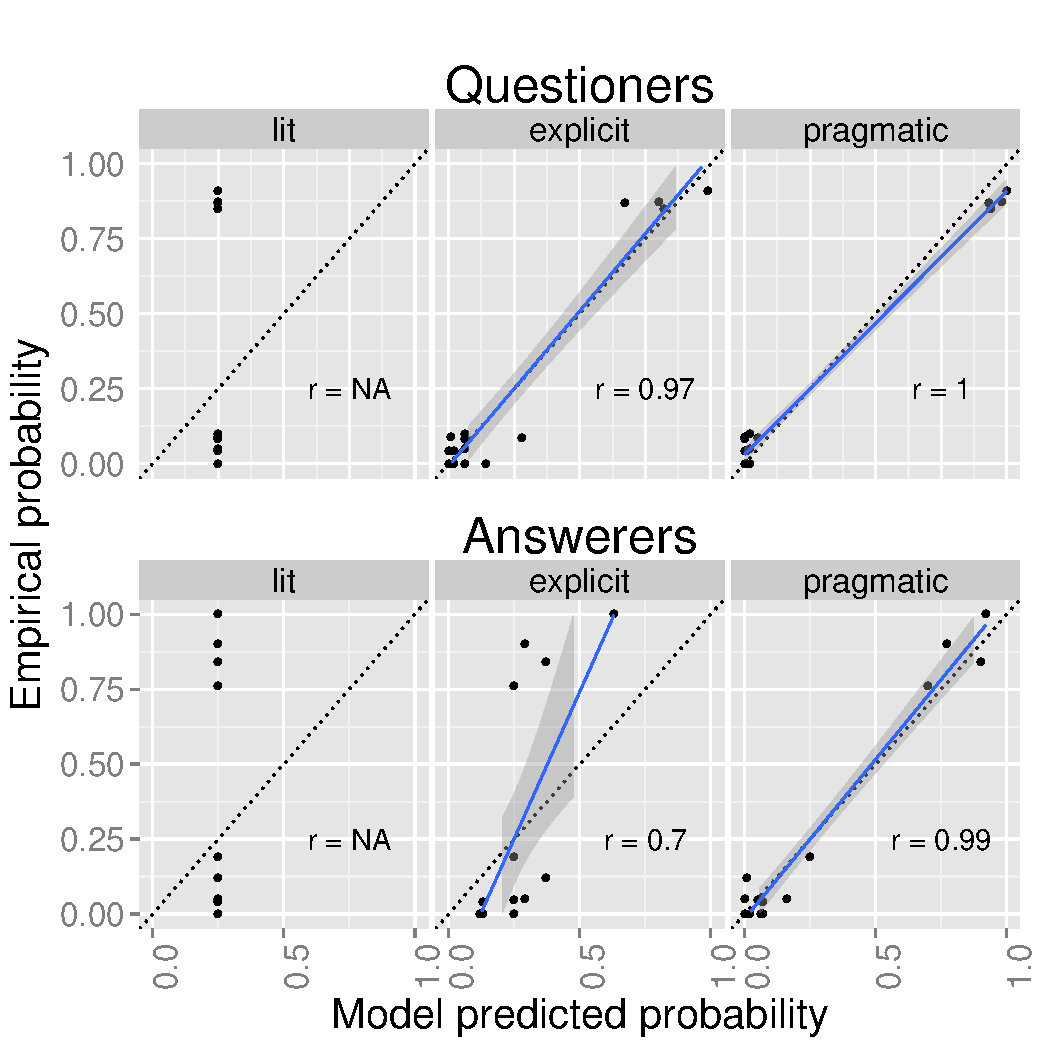
\includegraphics[scale=.75]{Exp3ModelFits.pdf}
\end{center}
\vspace{-.5cm}
\caption{Full space of models, and their correlations with the data from Exp.~1. Questioner models in the first row reason about the answerers directly below them, and the pragmatic answerer reasons about the explicit questioner.}
\label{fig:Exp3ModelSpace}
\vspace{-.15cm}
\end{figure}
%

\subsubsection{Discussion}

%We replicated the results of experiment 1 in a real-time, interactive setting. Again, we found that both explicit and pragmatic questioner models provide an excellent fit to questioner behavior, and that the pragmatic answerer accounts for the data significantly better than the explicit answerer both quantitatively and qualitatively. In addition, the full, interactive game was designed to be more natural and less confusing to participants than the drop-down menu design from experiments 1 and 2. Because players received constant feedback from their partner, this task was framed as inherently social, and because answerers watched as questioners moved words to form questions, there was a convincing mechanism for people to believe they were playing with another human. This addresses some concerns raised with experiments 1 and 2. 
Only the pragmatic answerer can account for essential qualitative features of the response data. For example, the explicit answerer predicts that participants will be equally likely to show the `dalmatian,' `poodle,' and `cat' when asked about a pet. Instead, the data show a significant preference for revealing the cat, leaving `dalmatian' and `poodle' at the same level as the other alternative. The pragmatic answerer correctly predicts this pattern  (see Fig.~\ref{fig:exp1res} (right)). Even more dramatically, the explicit answerer predicts a uniform distribution over responses to the `animal?' question. %(since all four responses denote animals)
However, the empirical distribution was significantly different from uniform. Thus, the pragmatic answerer is necessary to account for these data.

These data provide strong evidence for a pragmatic answerer, but are more equivocal with respect to the explicit and pragmatic questioner. Because the two models did not make significantly different predictions for this experiment (and both work quite well), we ran a follow-up study on a special case of the guessing-game paradigm in which the explicit and pragmatic questioners make different predictions.

Note that so far we have used the same animal hierarchy for the stimulus set in all our experiments, providing only 16 points of comparison between our models and empirical data. Furthermore, there exists a heuristic strategy for selecting questions given goals in the hierarchy structure we have been using which produces the same pattern of responses without requiring any social inference. Suppose questioners saw their goal on a given trial and ruled out labels that do not apply (e.g. a `cat' is neither a `dalmatian' nor a `dog'), then picked the most specific of the remaining labels (`pet' picks out a smaller set of objects than `animal'). Whether through use of this heuristic strategy or pragmatic inference (as our model suggests), questioners strongly converged on a single mapping from goals to question utterances. Because response probabilities are clumped at the ends of the scale, our fits to the questioner model are not particularly meaningful: we're fitting endpoints.
 
In experiment 2, we test the generality of our model by expanding the stimulus set to encompass multiple stimulus domains and multiple hierarchy structures designed to elicit graded judgements. This addresses the potential concern that the behavioral patterns we have been modeling are specific to the set of four animals or the tree-like hierarchy in which they were embedded. We also took care to include one simple but critical hierarchy structure where (1) the explicit and pragmatic questioner models make different predictions and (2) the heuristic strategy cannot mimic these predictions. 

\section{Exp.~2: Generalizing Predictions}

\subsubsection{Participants} We recruited 199 participants
from Amazon's Mechanical Turk to participate in this task. Fifty participants were excluded due to a server crash that terminated the task before completion. Two additional participants were excluded because they were not non-native English speakers. This left 74 unique completed games.


\subsubsection{Stimuli \& Procedure} A set of twelve items were created by crossing four domains (animals, plants, places, and artifacts) with three hierarchy structures (``branching'', ``overlapping'', and ``equivocal''; see Figure \ref{fig:hierarchyStructures}). For each item, there was a set of four goal objects in $\mathcal{G}$, which appeared on the wheel for the questioners, four question labels in $\mathcal{Q}$ that the questioner could use to ask about their assigned goal, and four answers in $\mathcal{A}$ corresponding to the four items in $\mathcal{G}$ that appear on the wheel.\footnote{A document containing these mappings for all items, as well as their hierarchical relationships, is available online at \url{https://github.com/hawkrobe/Q\_and\_A/blob/master/MultiExperiment2/stimuliLabels.pdf}} 

	\begin{figure}[t!]
\begin{center}
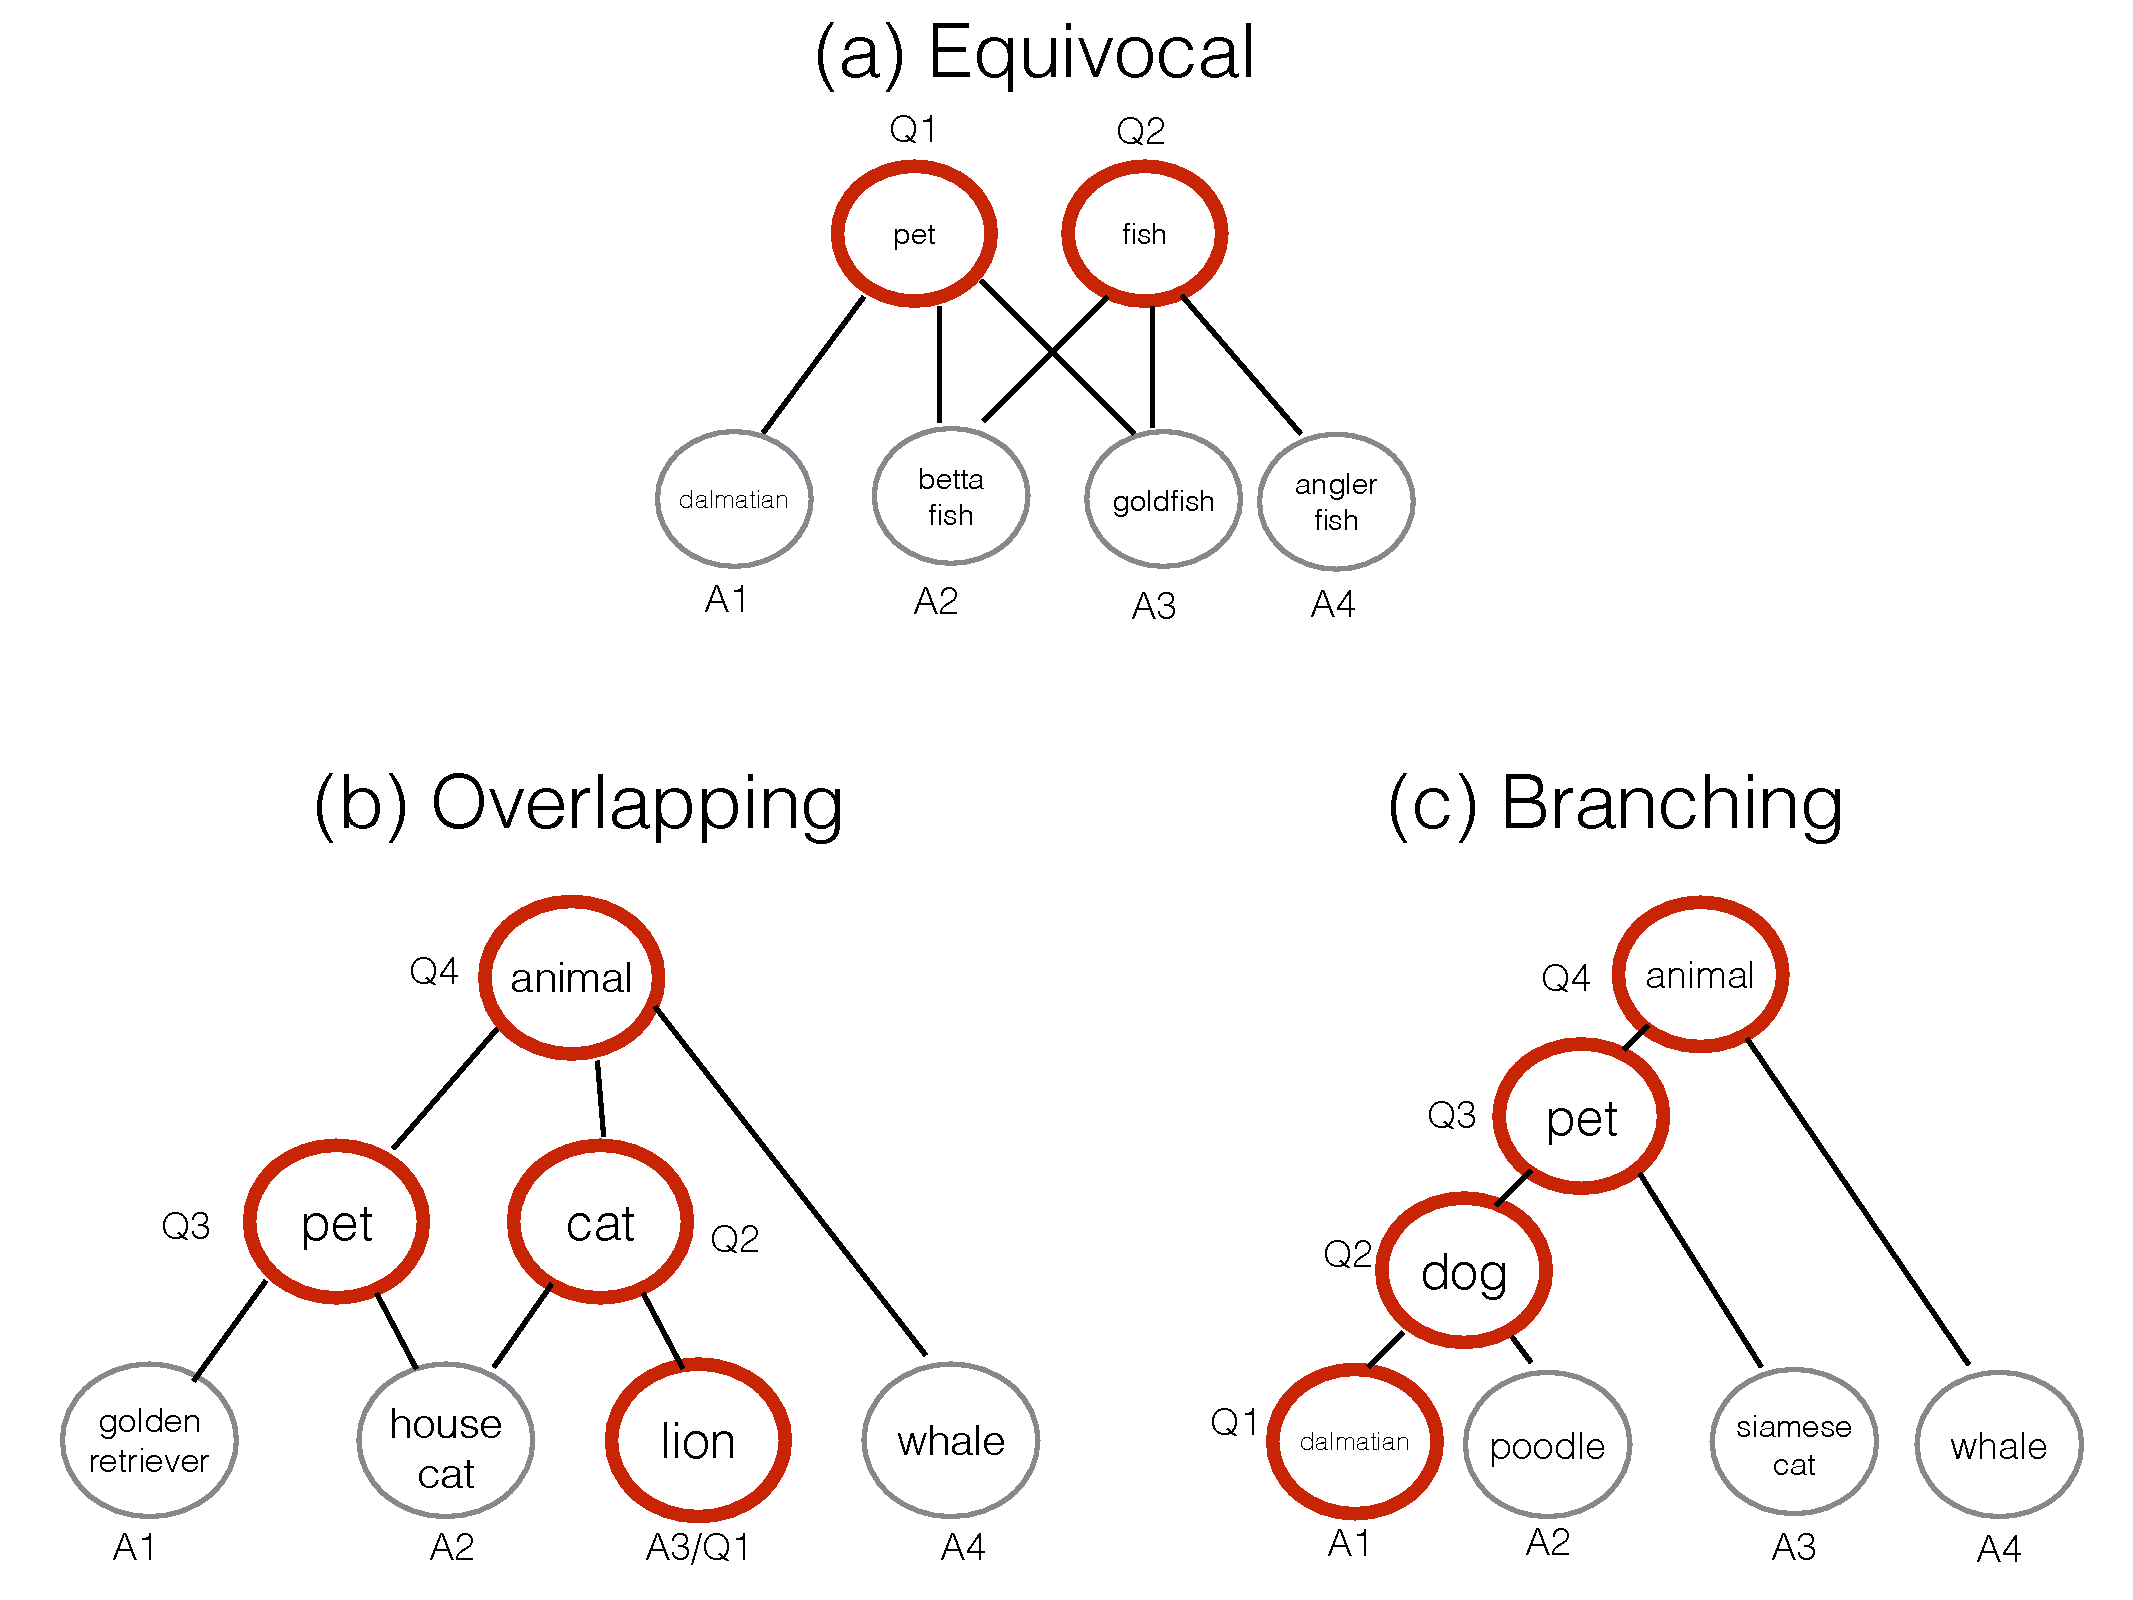
\includegraphics[scale = .3]{hierarchyStructureExamples}
\end{center}
\vspace{-.5cm}
\caption{Example of each type of hierarchy used in Experiment 4. The bottom row served as the answer space, and the labels in the questioner space highlighted in red. }
\vspace{-.1cm}
\label{fig:hierarchyStructures}
\end{figure}
The procedure was the same as Experiment 3 with two major modifications. First, we addressed an asymmetry in the task: the answerer watched the questioner move words, but the questioner only saw template text responses in response. In pilot work, we found that answerers were more likely to believe they were playing with a  human partner than questioners. To bring questioner and answerer beliefs closer together, we changed the mechanism by which the answerer responds. Instead of clicking on a gate and then clicking the `send' button, we supplied a ``Reveal Box.'' When the answerer was ready to reveal a gate, they would simply click and drag the object they wanted to reveal into this box. The questioner watched as the outline of the gate moved, in real time, and saw the image as soon as the answerer dropped it in the box. 

	\begin{figure}[t!]
\begin{center}
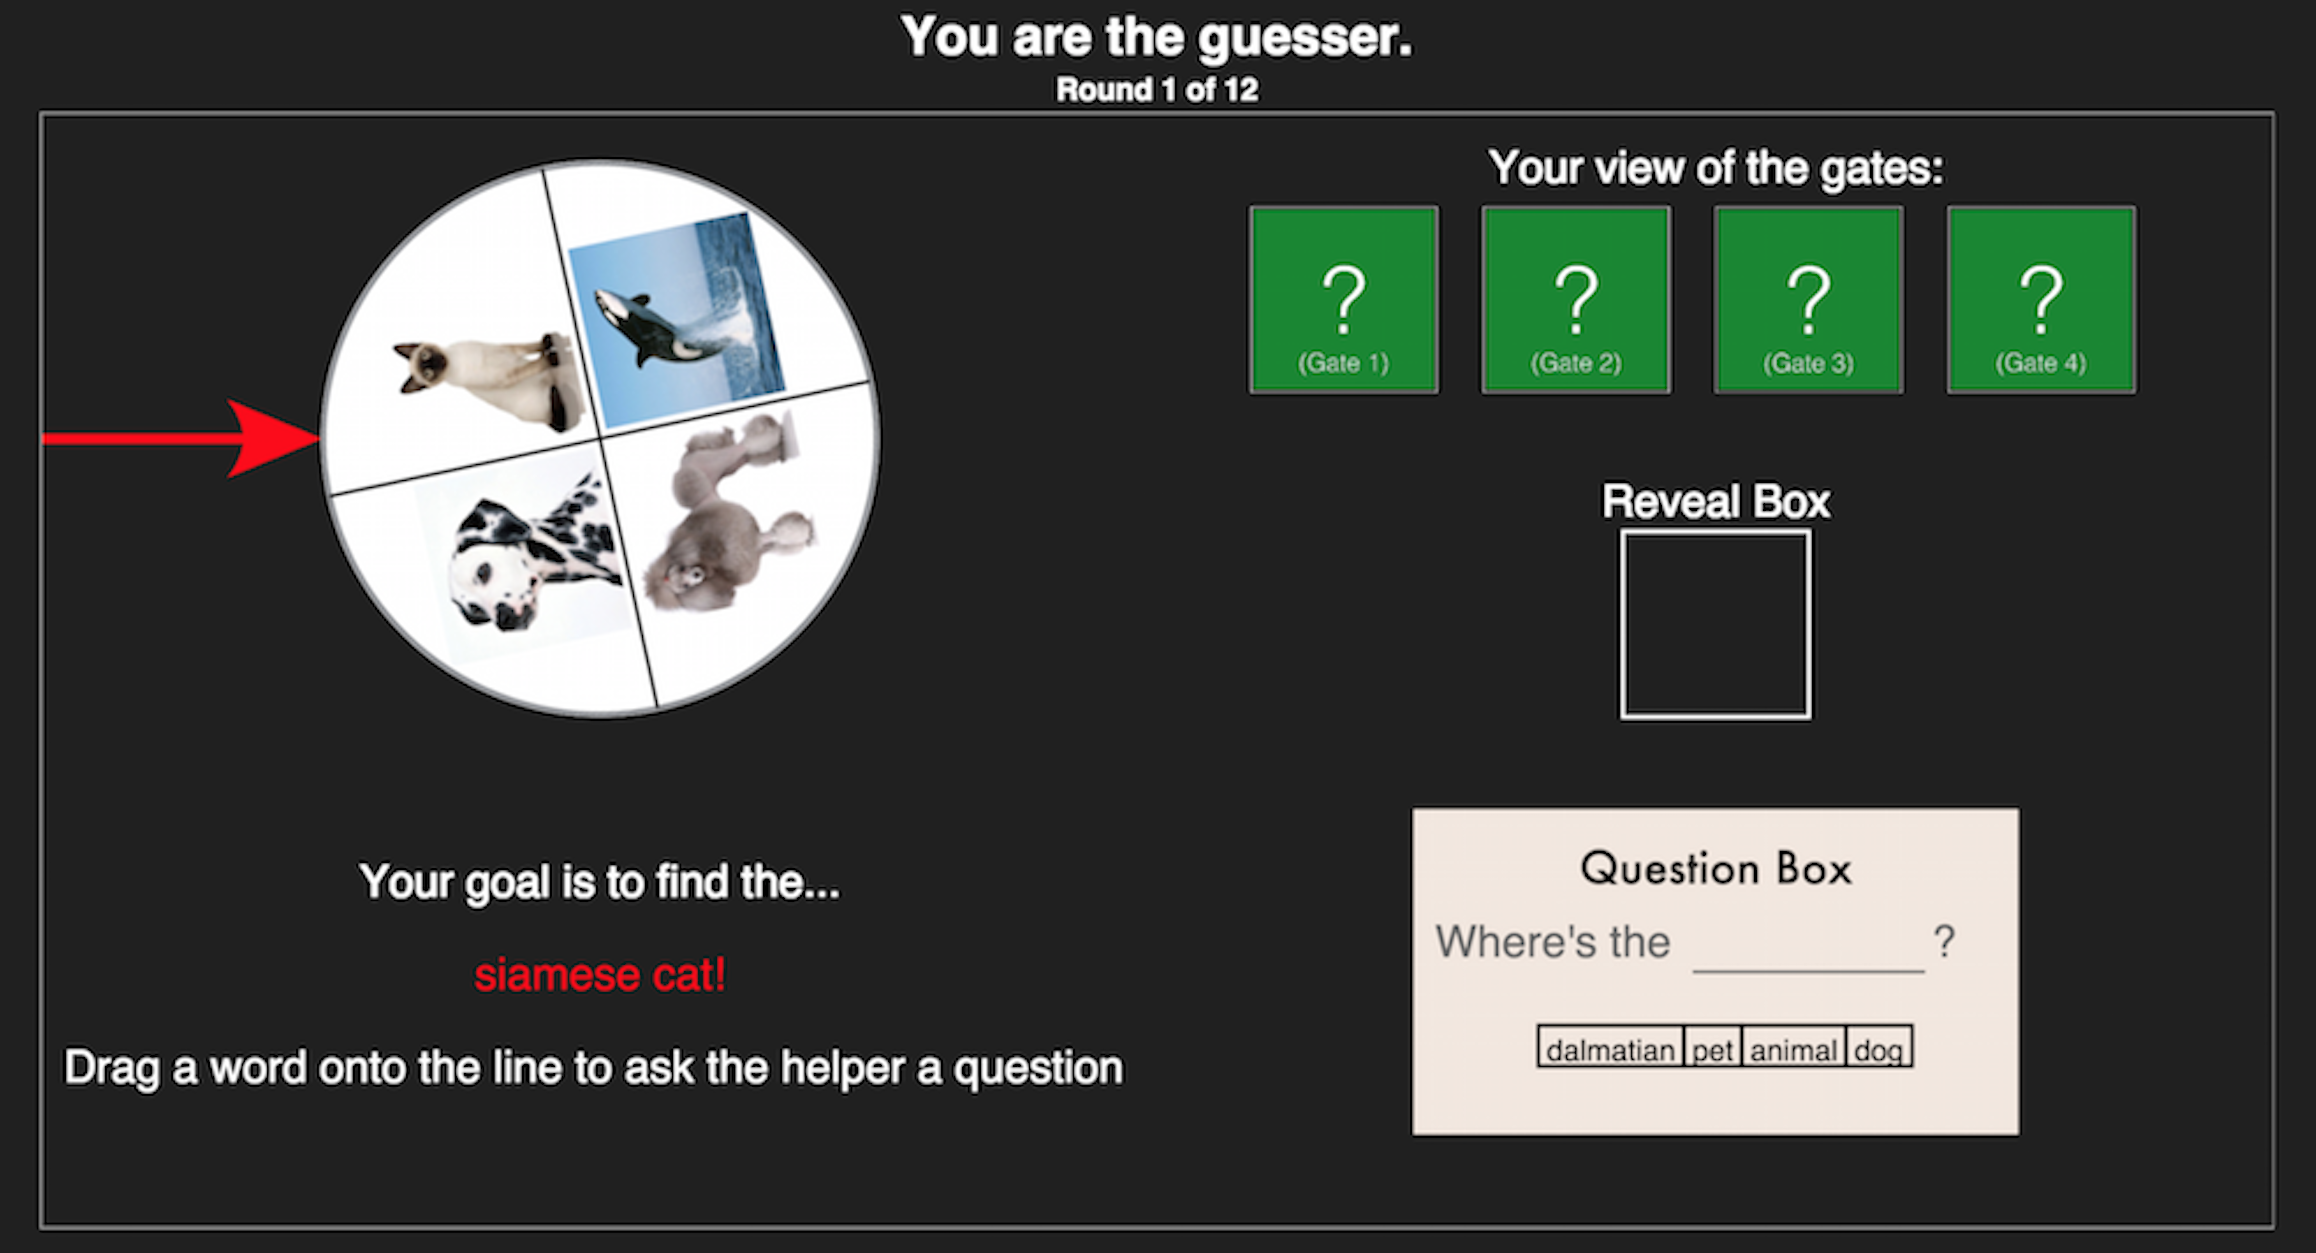
\includegraphics[scale = .3]{Exp4GuesserViewStart}
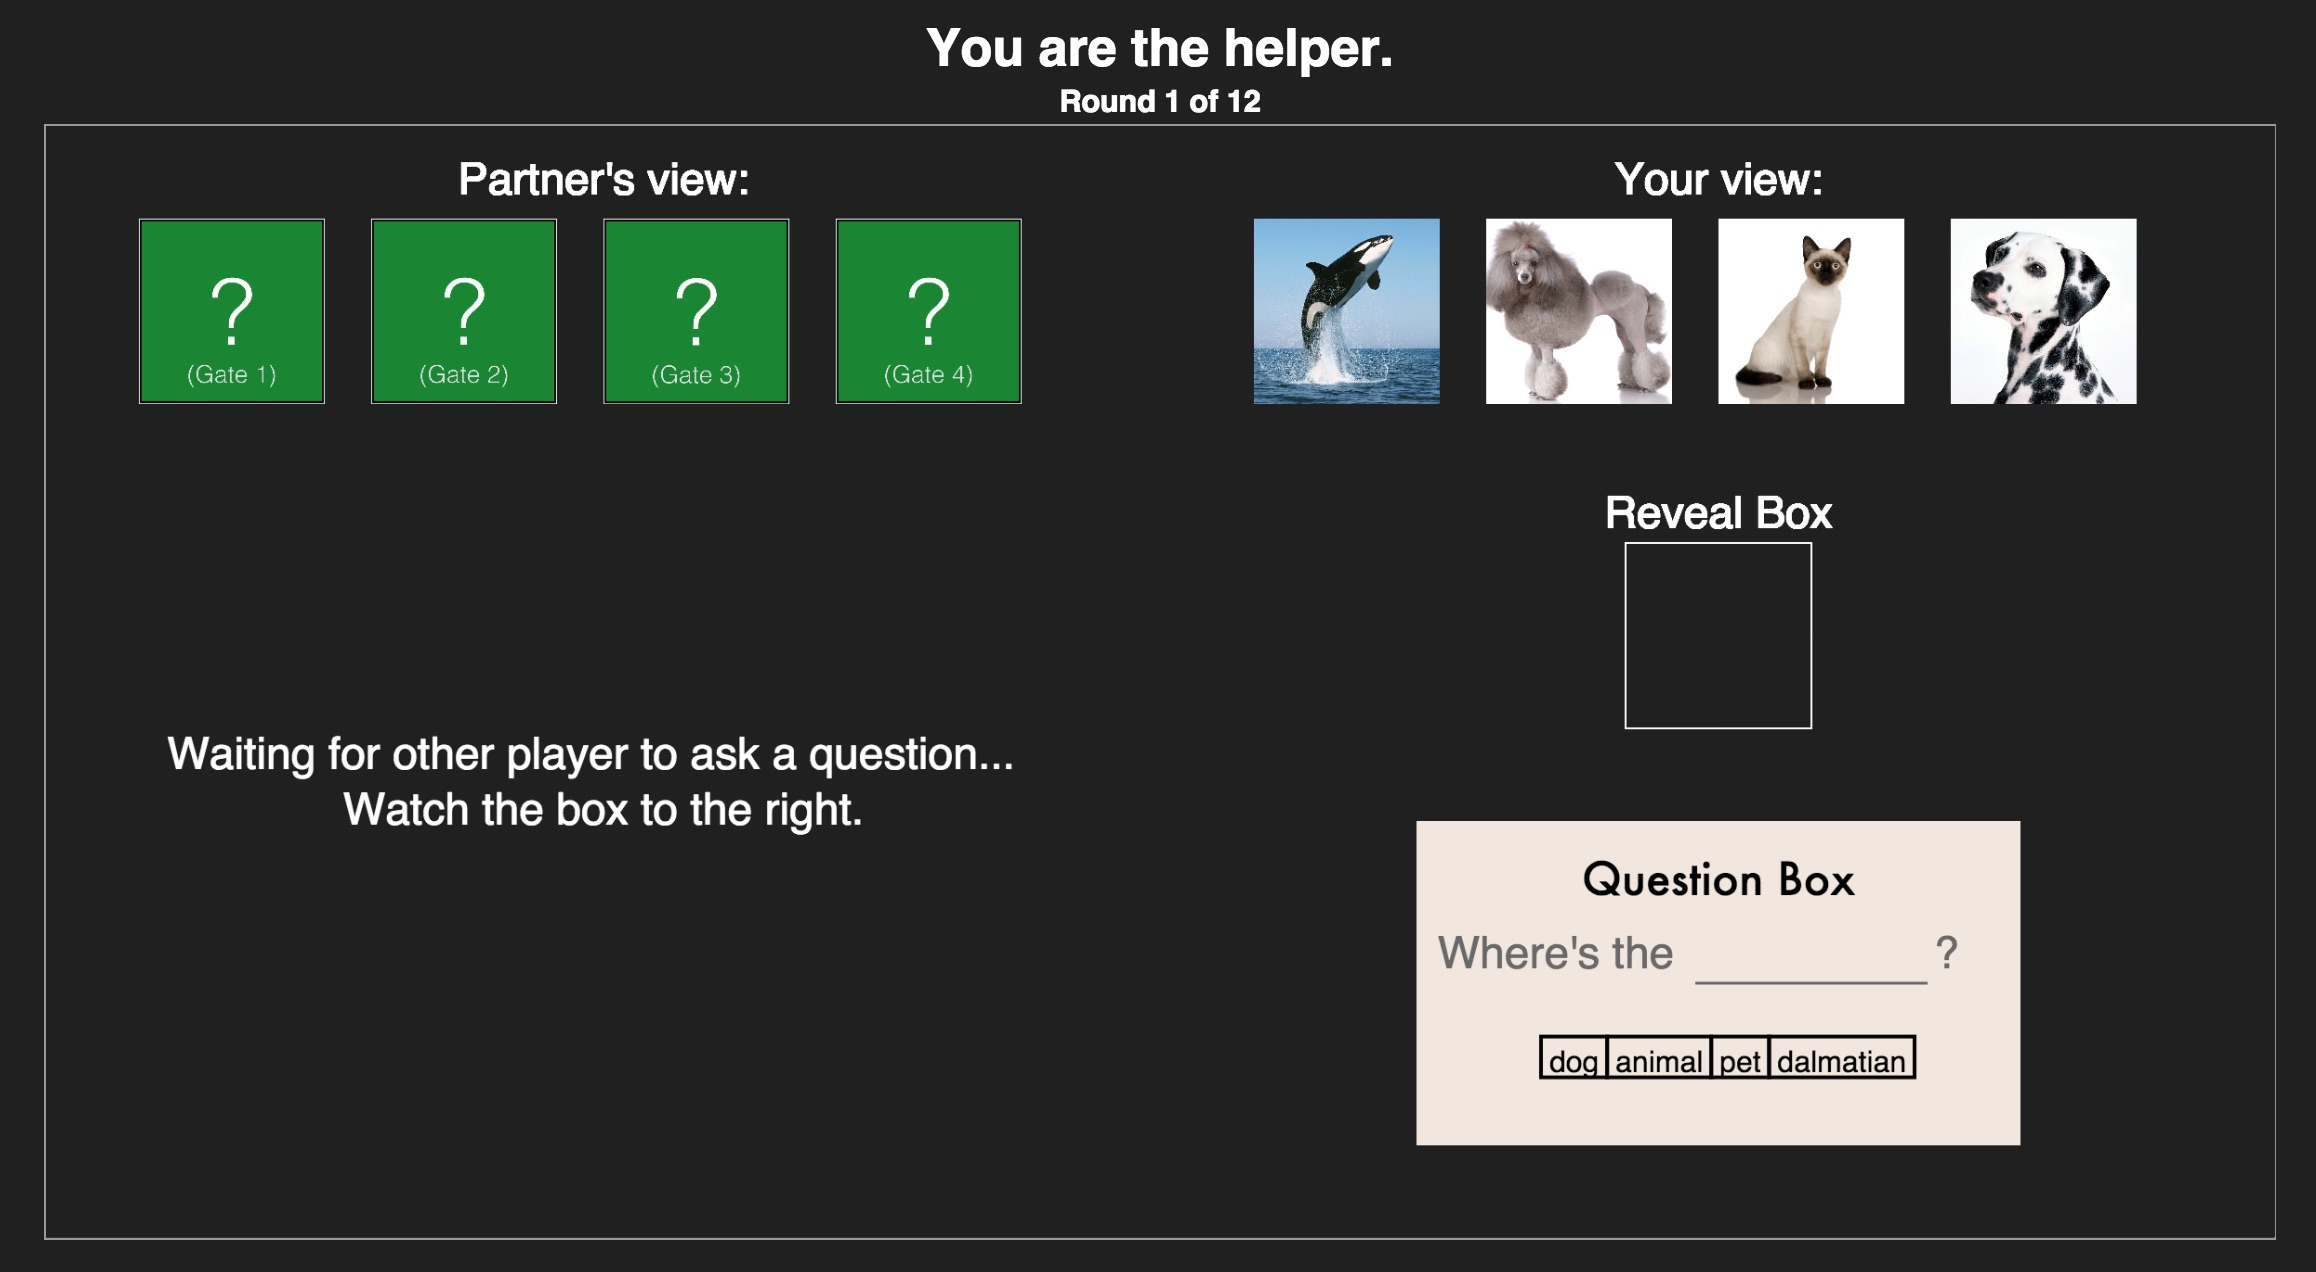
\includegraphics[scale = .15]{Exp4HelperViewStart}
\end{center}
\vspace{-.5cm}
\caption{Exp.~4 interfaces, for the questioner (top) and answerer (bottom).}
\vspace{-.1cm}
\label{fig:exp4views}
\end{figure}

Second, we noticed that some players began exploiting the freedom of the ``question box'' drag-and-drop procedure after playing several rounds. On difficult items, especially those in the equivocal hierarchy where our model predicts no preferred question for certain goals, players would use the words to form non-grammatical signals. This is interesting behavior in its own right, but we are interested in testing models which operate over a well-defined set of question utterances held in common ground. We therefore pre-set a frame ``Where is the \dots'' for the question box and allowed participants to drag one and only one of the question labels into the blank. 

The resulting questioner and answerer interfaces are displayed in Figure \ref{fig:exp4views}.  Each participant provided one response for each of the twelve items, presented in random order. 

\subsubsection{Results}

First, we note that there was high correlation in response probabilities across domains for both questioners and answerers (see Table \ref{table:experiment4correlations}). Thus, in examining the results below we will collapse across domains for simplicity of analysis. Still, it is worth noting that the ``place'' domain has the lowest inter-domain correlations for both questioners and answerers, indicating that it may be an outlier -- we will return to this point in the discussion below.  Next, we step through the response patterns for each hierarchy type. For concreteness, though all statistical tests were conducted on data pooled across domains, we report our results in terms of the `animal' domain instead of the abstract goal, question, and answer labels (see Figure \ref{fig:exp4res} for the full response distributions).

In the `equivocal' condition (Figure \ref{fig:hierarchyStructures}(a)), the questioner chose whether to ask about the `pet' or the `fish'; two of the goal animals were `pet fish' belonging to both categories, while the other two animals were just a pet (e.g. a dalmatian) or just a fish (e.g. a deep-sea angler fish), respectively. We found that when trying to find the object that was only a pet or only a fish, participants preferred to ask `pet', $\chi^2(1) = 67, p < 0.001$, or `fish,' $\chi^2(1) = 57, p < 0.001$, respectively. Answerers, in turn, revealed the location of the `dalmatian' when asked about the `pet', $\chi^2(3) = 238, p < 0.001$, and the location of the `angler fish' when asked about the `fish,' $\chi^2(3) = 142, p < 0.001$. 

For the two objects belonging to both categories, where we expected questioners to have no preference, we found strong variability across domains -- in the `animal' domain, for example, 85\% of questioners asked about the `fish' when given one of the `pet fish' goals, compared to only 15\% asking about the `pet,' $\chi^2(1) = 15, p < 0.001$. In the `artifacts' domain, on the other hand, questioners had no preference between asking about the `seat' or `metal thing' when the objects (metal chairs) fell into both categories, $\chi^2(1) = 0.4, p = 0.52$. This suggests that labels have differential fitness when applied to different objects, and participants are relying on more knowledge than the purely structural connections captured by the hierarchy. 

In the `overlapping' condition (Figure \ref{fig:hierarchyStructures}(b)), questioners preferentially asked about the `lion' when looking for the lion, $\chi^2(3) = 205, p < 0.001$; about the `cat' when looking for the Siamese cat, $\chi^2(3) = 63, p < 0.001$, even though the lion is also a cat; about the `pet' when looking for the dalmatian, $\chi^2(3) = 232, p < 0.001$, even though the Siamese cat is also a pet; and about the `animal' when looking for the whale, $\chi^2(3) = 213, p < 0.001$. Answerers preferentially revealed the lion when asked about the `lion,' $\chi^2(3) = 229, p < 0.001$, the Siamese cat when asked about the `cat,' $\chi^2(3) = 59, p < 0.001$, the dalmatian when asked about the `pet,' $\chi^2(3) = 120, p < 0.001$, and the whale when asked about the `animal,' $\chi^2(3) = 187, p < 0.001$. 

In the `branching' hierarchy (Figure \ref{fig:hierarchyStructures}(c)), we replicated our findings from Experiments 1 and 3 with a broader set of items: questioners strongly prefer to ask about the `dalmatian' when trying to find the dalmatian, $\chi^2(3) = 190, p < 0.001$, about the `dog' when trying to find the poodle, $\chi^2(3) = 152, p < 0.001$, about the `pet' when trying to find the siamese cat, $\chi^2(3) = 168, p < 0.001$, and about the `animal' when trying to find the whale, $\chi^2(3) = 210, p < 0.001$. Answerers behave identically to previous experiments, $p < 0.001$.

\begin{table}[b]
\centering
\begin{tabular}{ p{1.5cm} | r | r | r | r |||||| r | r | r | r |}
& \multicolumn{4}{c||||||}{Questioners} & \multicolumn{4}{c}{Answerers} \\
&             animal &     place &     plant &  artifact &            animal &     place &     plant &  artifact \\
\hline
animal &   1.00 &  0.91 & 0.94 & 0.94 & 1.00 & 0.78 & 0.92 &  0.97 \\
\hline
place &    0.91 &  1.00 & 0.96 & 0.95 & 0.78 & 1.00 &  0.78 & 0.78 \\
\hline
plant &    0.94 & 0.96 & 1.00 & 0.97 & 0.92  & 0.78 &  1.00 & 0.91\\
\hline
artifact & 0.94 & 0.95 & 0.97 & 1.00 & 0.97 & 0.78 &  0.91 & 1.00\\
\end{tabular}
\\[1.5pt]
\caption{Inter-domain correlations in Experiment 4} 
\label{table:experiment4correlations}
\end{table}

\begin{figure}[t!]
\begin{center}
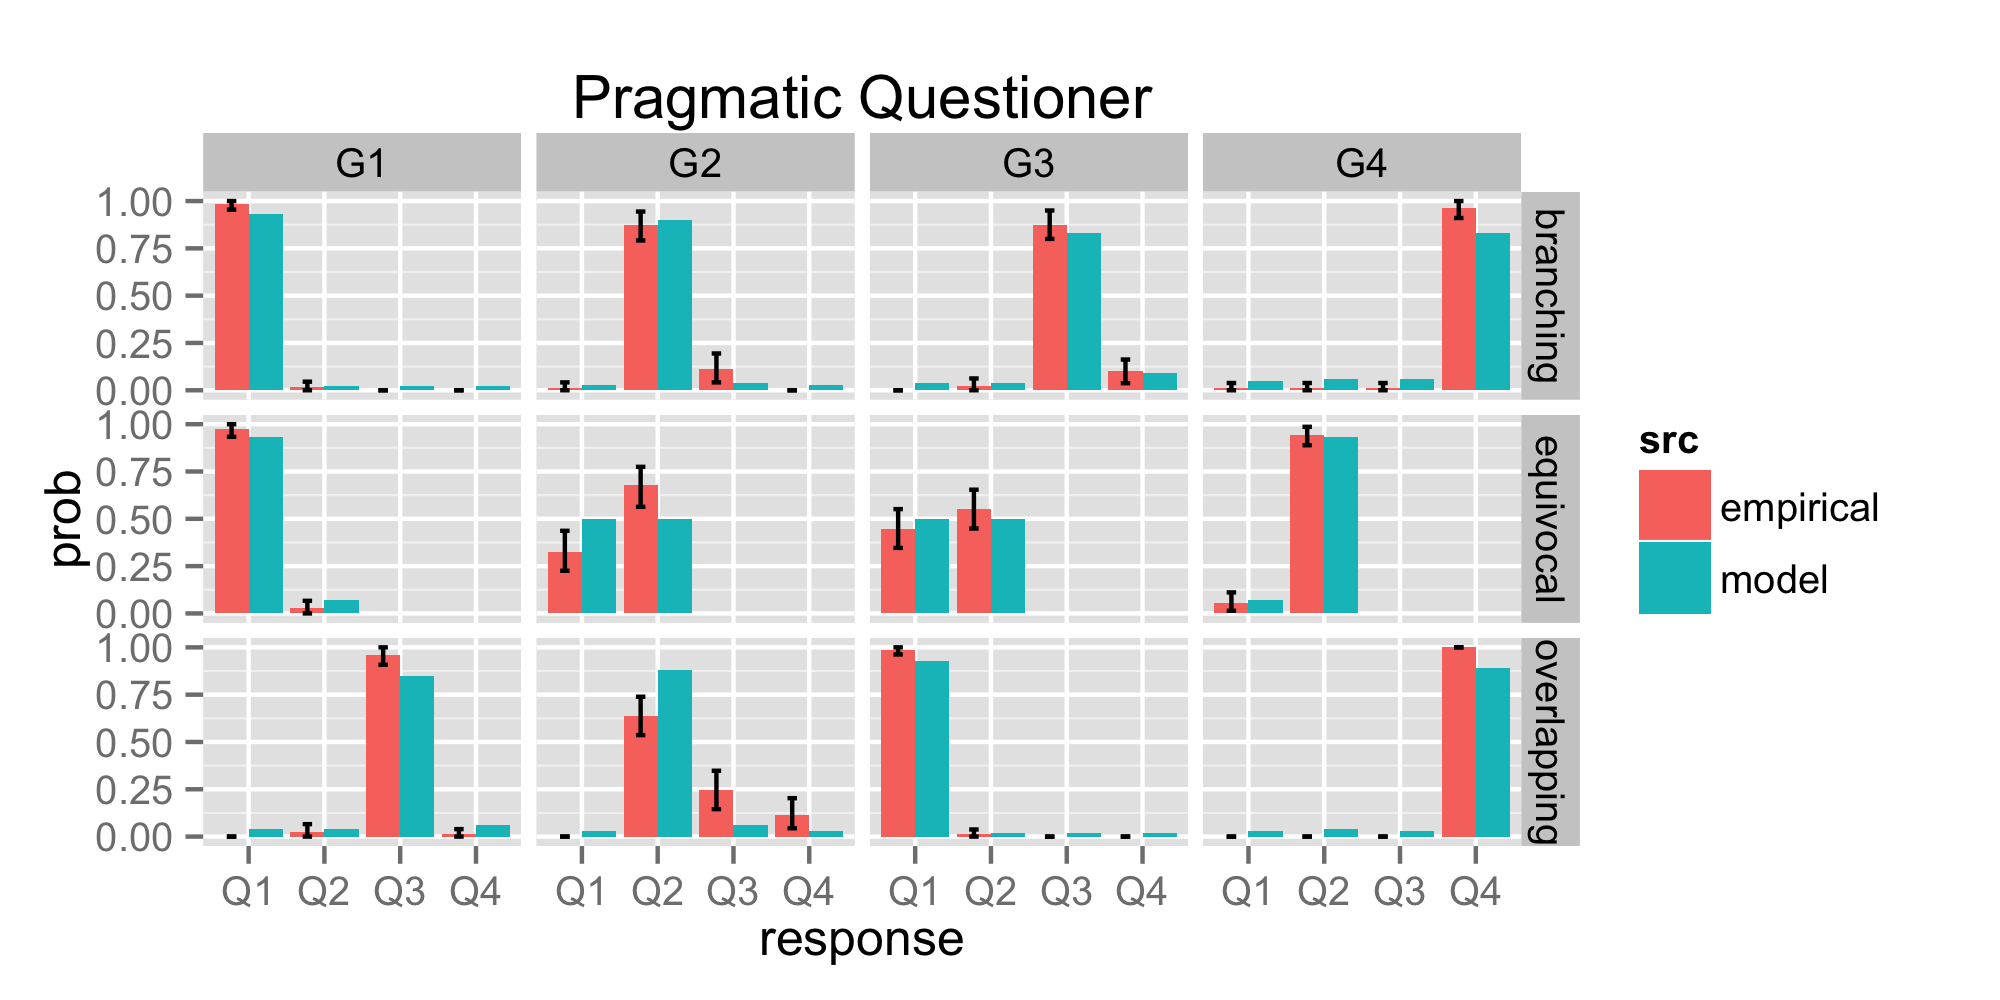
\includegraphics[scale = .25]{Exp4QuestResults}
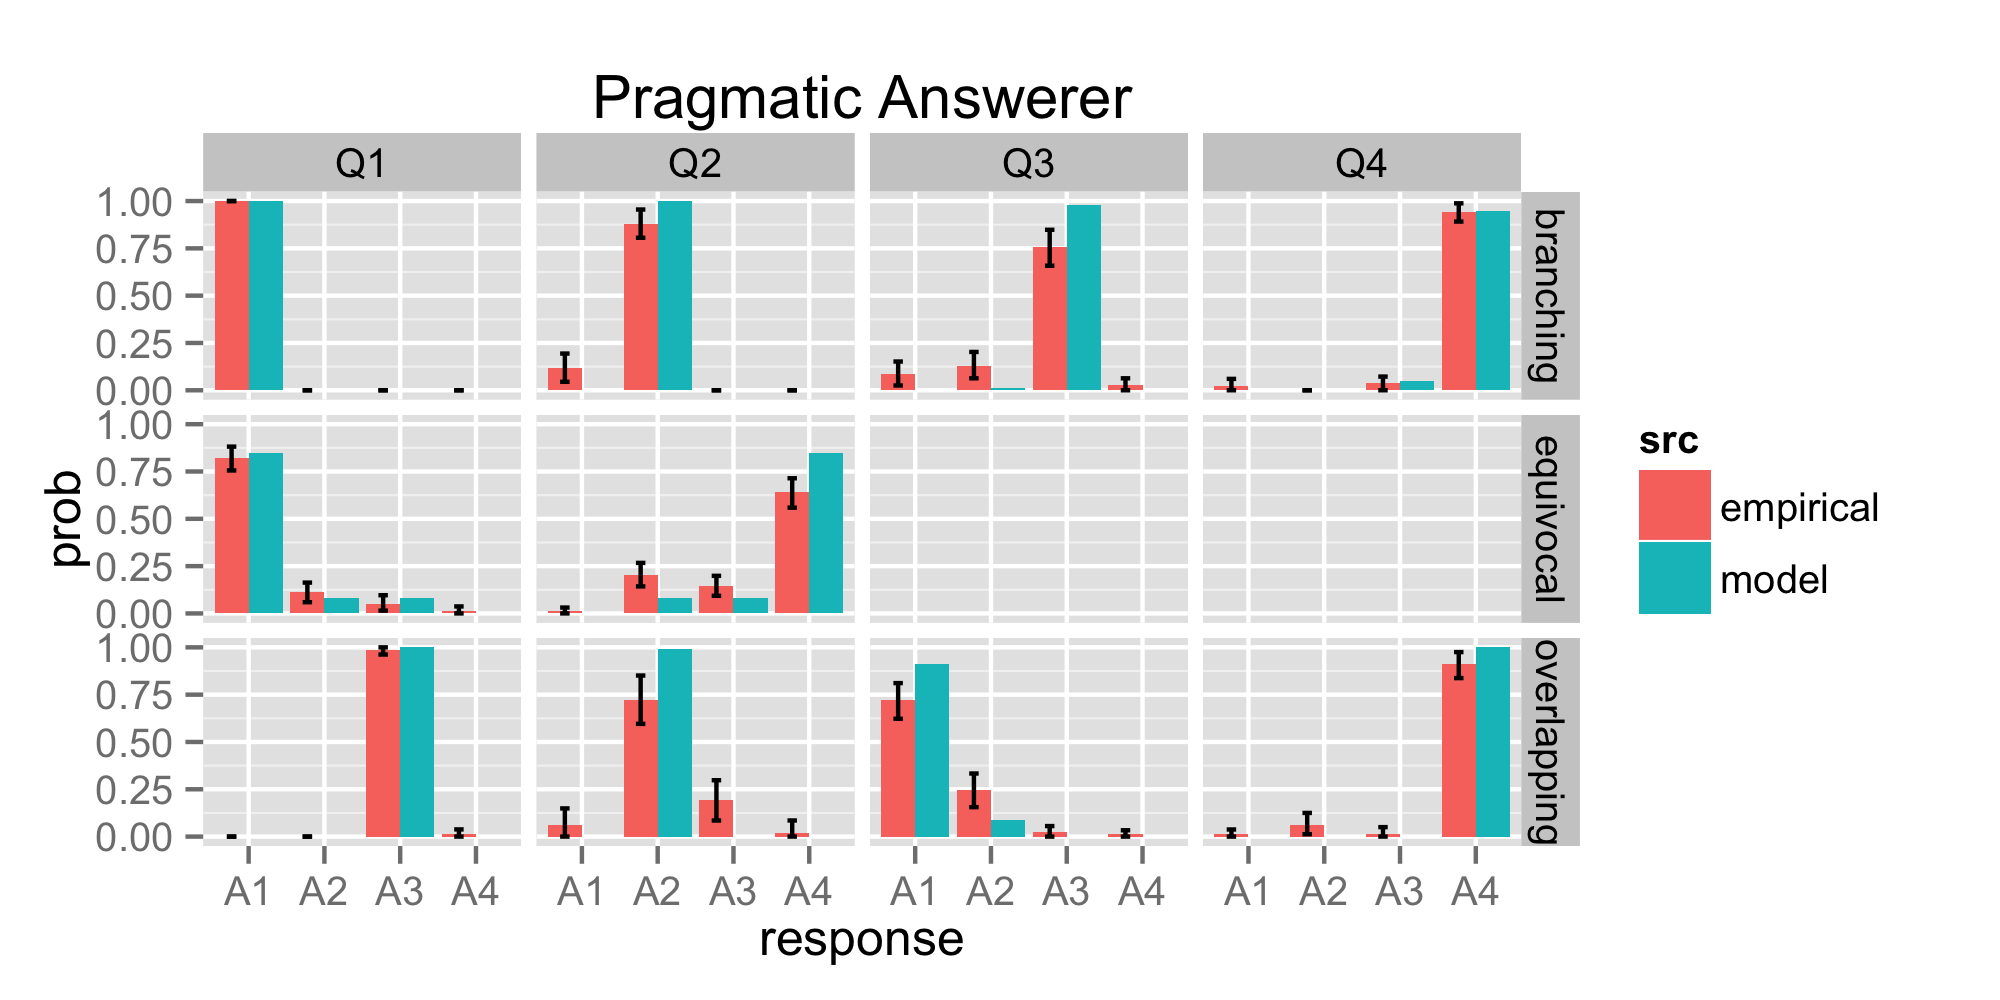
\includegraphics[scale = .25]{Exp4AnsResults}
\end{center}
\vspace{-.5cm}
\caption{Exp.~4 results and model fits, for the best-performing questioner (left) and answerer (right) models, collapsing over the different domains. Error bars represent bootstrapped 95\% confidence intervals.}
\vspace{-.1cm}
\label{fig:exp4res}
\end{figure}

\subsubsection{Model comparison}

%
\begin{figure}[t!]
\begin{center}
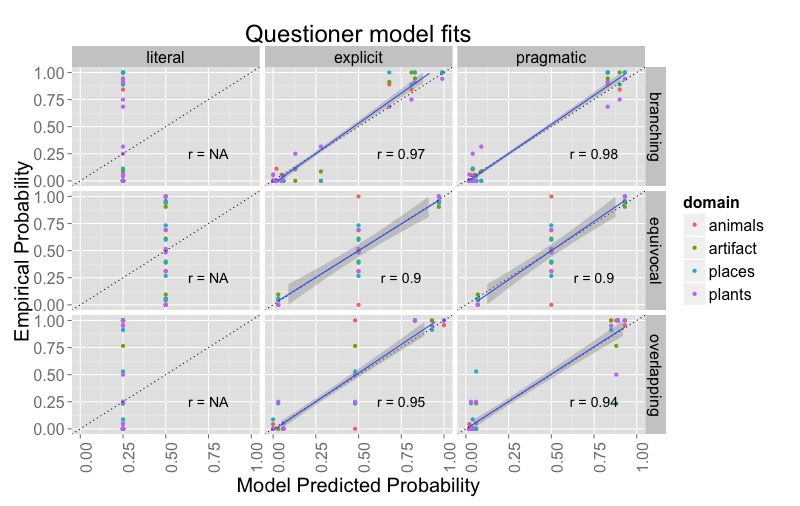
\includegraphics[scale=.55]{Exp4QuestFits.jpeg}
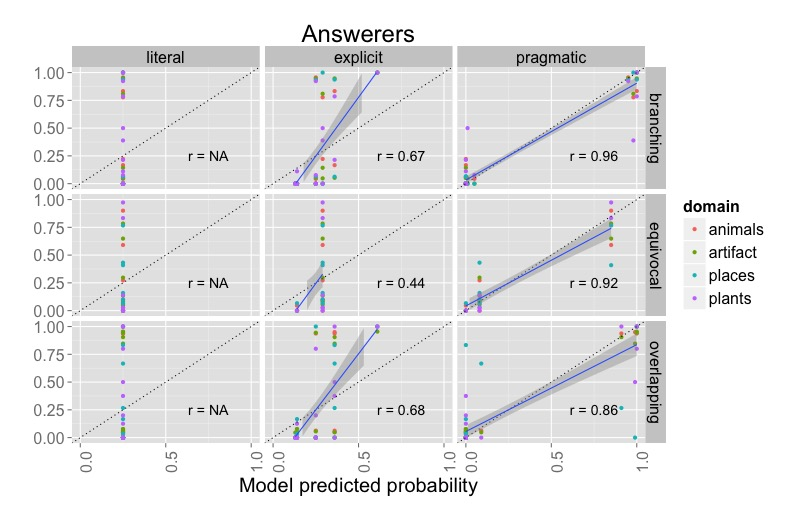
\includegraphics[scale=.55]{Exp4AnsFits.jpeg}
\end{center}
\vspace{-.5cm}
\caption{Full space of models, and their correlations with the data from Exp.~4, broken down by item and type.}
\label{fig:Exp4ModelSpace}
\vspace{-.15cm}
\end{figure}
%

Model comparison was conducted in the same way as in Experiment 1 and 3. However, to avoid overfitting and to reduce the number of free parameters that would result from separately fitting rationality parameters for each item, we pool together data from all hierarchy structures and domains and fit the single rationality parameter for each model to jointly optimize model-data correlations across all items in this pooled dataset. 

These model-data fits, broken down by model level and hierarchy structure, are displayed in Figure \ref{fig:Exp4ModelSpace}. We can immediately rule out the literal answerer and literal questioner, which predict a uniform distribution of responses. We also find that the explicit answerer models fit the data significantly worse than the pragmatic answerer model in all hierarchy structures, with $r = 0.67$ compared to $r = 0.96$ in the `branching' hierarchy, $r = 0.44$ compared to $r = 0.92$ in the `equivocal' hierarchy, and $r = 0.68$ compared with $r = 0.86$ in the `overlapping' hierarchy, respectively. 

Turning to the questioner predictions, we again find that both explicit and pragmatic models provide excellent but essentially indistinguishable fits, with $r = 0.97$ compared with $0.98$ in the `branching' hierarchy, $r = 0.90$ compared with $r = 0.90$ in the `equivocal hierarchy', and $r = 0.95$ compared with $0.94$ in the `overlapping' hierarchy, respectively. 

However, because we designed the overlapping structure to provide a critical test for the questioner models, it is not the overall correlation we are interested in, it is the particular distribution of responses to ``G2'' (the ``house cat'' in the animal domain). Since ``house cat'' is not available as a question, the explicit model (as well as the heuristic strategy discussed above) predicts that the two parents, ``pet'' and ``cat'' will be equally likely. This happens because the explicit answerer would be equally likely to reveal the location of the house cat in response to ``pet'' and ``cat,'' which each have two children. 

The pragmatic questioner model, however, predicts that ``cat'' will be preferred over ``pet'', because the other child of ``cat'' -- the lion -- is pragmatically blocked by the pragmatic answerer. When the pragmatic answerer hears ``cat'' they reason that if the questioner's underlying goal were the ``lion'' they would have \emph{said} lion; because they didn't, they must mean the other cat. Thus, we have a pair of sharply distinguishable predictions: the explicit model predicts that ``pet'' and ``cat'' will be equally likely and the pragmatic model predicts an asymmetry where ``cat'' is the preferred label. 

In Figure \ref{fig:Exp4ZoomedIn}, we zoom in on this critical condition and display both models' predictions next to the empirical data, with bootstrapped 95\% confidence intervals. For these analyses, we excluded the `places' domain both because it was flagged as an outlier early in the analysis and because our stimulus design led to a confound in the `overlapping' condition, which we discuss further below. We find that the pragmatic model makes the correct qualitative prediction -- the mean probability of responding ``Q2'' ($p_{Q2} = 0.77, n = 52, 95\%\textrm{ bootstrapped CI }= [0.65, 0.88])$ in this condition is significantly different from the mean probability of responding ``Q3'' ($p_{Q3} = 0.15, n = 52, 05\% \textrm{ bootstrapped CI }=[0.06, 0.25]$), as predicted by the pragmatic model. We also see that it makes a relatively good quantitative prediction, with the predicted probability lying within the 95\% confidence interval of the empirical estimate for both the ``Q2'' and ``Q3'' responses. Recall that a single free parameter $\alpha$ for each model was fit to maximize correlations for the entire (pooled) dataset.

%
\begin{figure}[t!]
\begin{center}
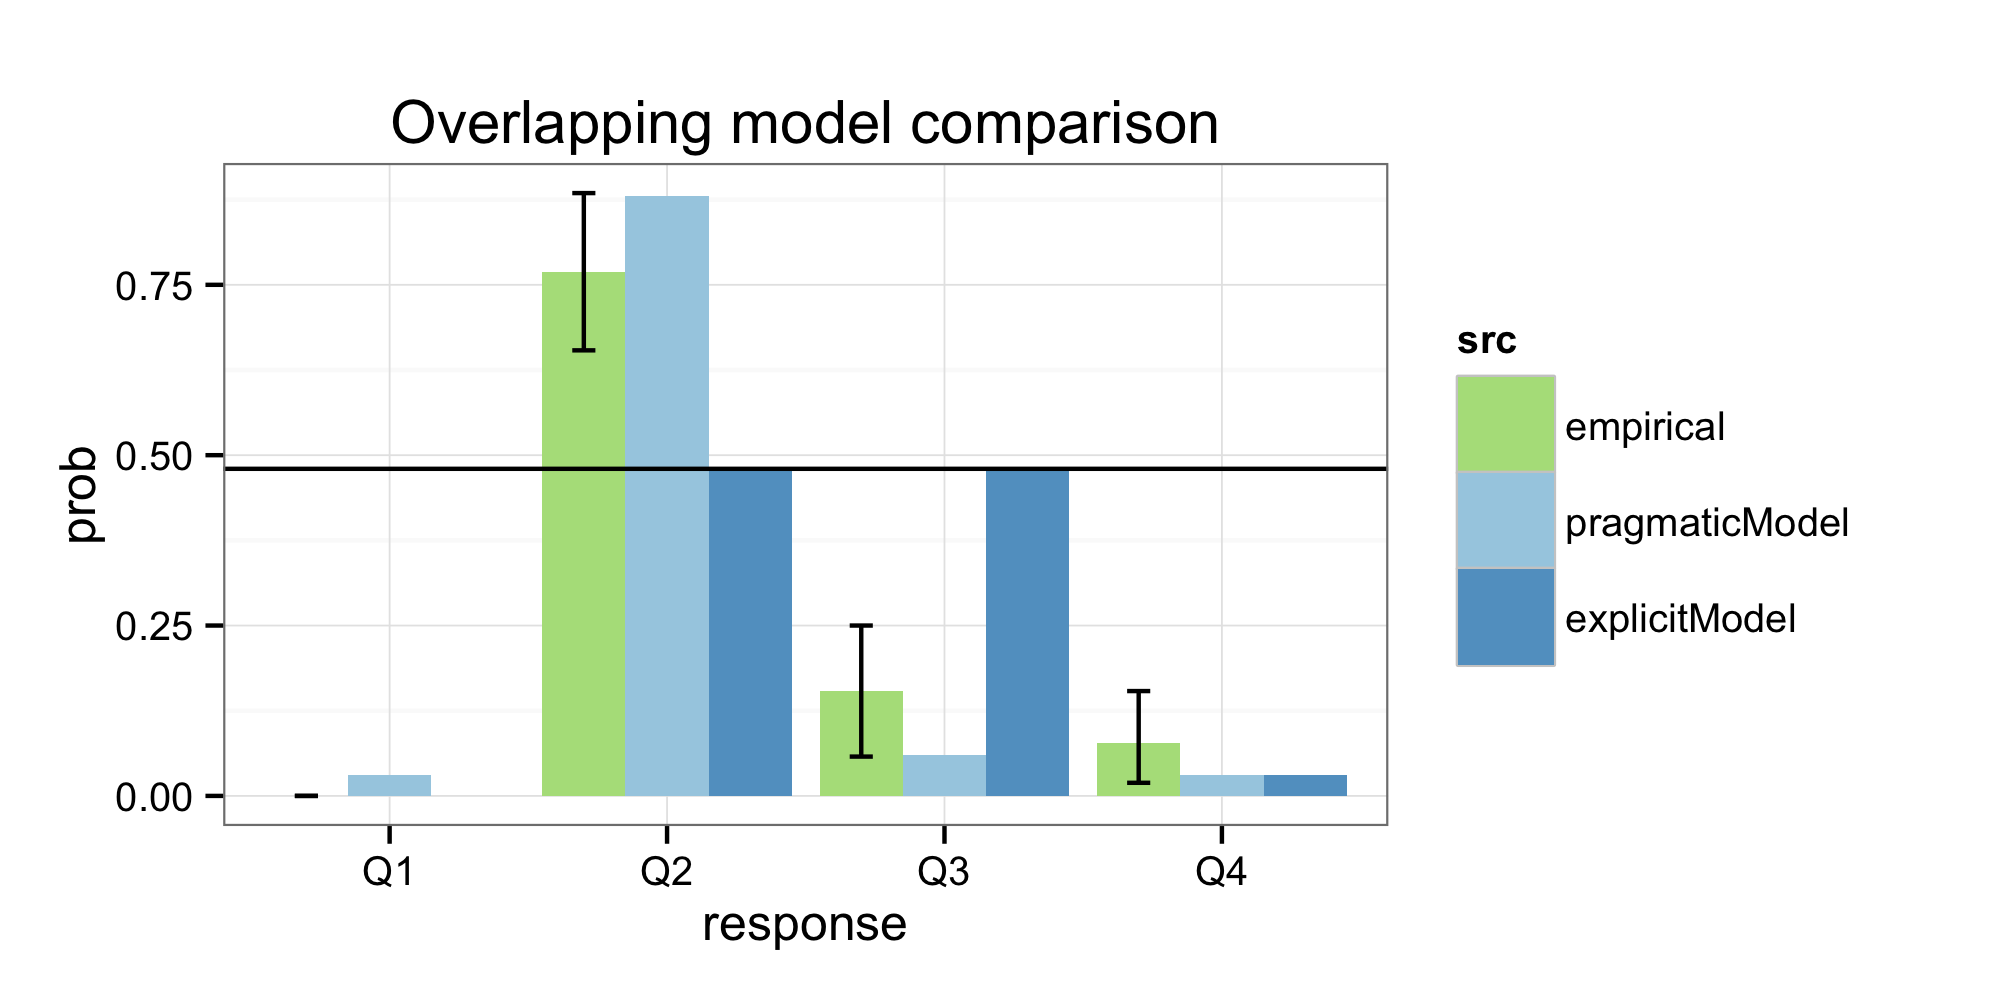
\includegraphics[scale=.25]{OverlappingModelComparison.png}
\end{center}
\vspace{-.5cm}
\caption{Full space of models, and their correlations with the data from Exp.~4, broken down by item and type.}
\label{fig:Exp4ZoomedIn}
\vspace{-.15cm}
\end{figure}
%


\subsubsection{Discussion}

We have again replicated the results of Experiments 1 and 3, and shown that these results generalize to a wider range of domains and hierarchy structures. Additionally, we were finally able to distinguish between the pragmatic and explicit questioner models, finding that the pragmatic model is necessary to account for some critical aspects of the data. The ``place'' domain that we flagged as a potential outlier earlier in the results is the only domain that does not show the pattern of responses predicted by the pragmatic questioner model. This is likely due to the choice of images displayed to participants: the two ``parent'' nodes of the critical goal are ``bar'' and ``restaurant,'' and we represented the intersection of these two categories as a hotel lobby. However, the image we chose placed emphasis in the bar in the hotel, which may have biased participants toward the ``bar'' response instead of the ``restaurant response'' predicted by the pragmatic model. Including it does not change the statistical results, but we do not believe it is representative of questioner behavior. 

\todo[inline]{The next paragraph would naturally lead into another experiment where we elicit label priors and re-run our model with label fitness included -- I think I'd be happier with the paper if we had this...}
We also find that while overall fits are good, all our models fail to capture graded responses across different domains. This is especially striking in the `equivocal' condition where all our models predict a symmetry in questioner behavior for the two goals where the questions options are equally uninformative. Instead, we found a high degree of variability across domains. To some extent, this is expected from a model with only a single parameter fit for all domains simultaneously. We could have fit separate rationality parameters for each domain to capture domain-level differences. However, we expect that this variability can be accounted for in a more principled way by a prior over label fitness. In our data, `fish' was considered a better label for a picture of a pet goldfish than `pet' by 85\% of participants, even though both are technically true. When there is no pragmatic reason to favor one over the other, participants fall back on their label prior. If we ran a separate study to elicit this prior, we could simply plug the empirical priors into our model and naturally account for the variability across items without introducing additional free parameters. Alternatively, we could use Bayesian data analysis to infer these priors from question and answer response data. 

\section{General discussion}
\label{sec:gd}

We have presented evidence that answerer behavior is best described by a pragmatic model that \emph{does} reason about questioner intentions, using the question utterance as a signal. Our study provides a next step for previous QUD-based linguistic accounts by concretely specifying how an answerer may make such inferences via Bayesian conditioning. The superiority of pragmatic answerer predictions over the other answerer models was robust across all experiments. 

Questioner behavior in Exp.~2, however, seemed to be much more dependent on experience. In another version of Exp.~1, we did not emphasize certain aspects of the game in the instructions, such as the fact that the answerer knows about the restricted answer set, which might prompt perspective-taking. 
Our data in this pilot experiment appeared to contain a mixture of explicit and pragmatic answerers and questioners (though other confounds were present in this version). We found the interactive, multi-player version of the task, used in Exp.~3 and Exp.~4 to be more robust to these minor variations. We also found that at least in certain scenarios like the overlapping hierarchy condition of Exp~.4, questioners systematically relied on higher-order pragmatic reasoning about what inferences an answerer would make about their own underlying goals when deciding what question to ask. Note that this behavior also could not be explained by the heuristic strategy raised in the earlier experiments: if questioners just ruled out labels that did not apply (e.g. ``lion''), they would have no mechanism for deciding between the two equally-good parent labels (``pet'' and ``cat'') to pick out their goal. It will ultimately be important to explore the mixture of explicit- and pragmatic-questioning across an even larger range of situations: these issues may be a product of our artificial game paradigm, or they may be reflective of real tendencies in language use, raising novel questions about audience design in question-answer behavior.

\todo[inline]{ndg: somewhere (discussion?) explore whether this notion of goals is enough.}

Perhaps the most important formal advance of the models considered here is to move the Rational Speech Act framework beyond interpretation of single utterances (in context), to consider the dynamics of simple dialogs (albeit consisting of a single question and its answer). 
Doing so requires replacing the immediate motive to convey true information with the more distant motive to provoke useful information from one's interlocutor. On the answerer side, sophisticated inference was required to account for the implicit interests of the questioner. This provides a useful connection to current game-theoretic and decision-theoretic models \cite{VogelBodoiaPottsJurafsky13_GricePOMDP, VanRooy03_QuestioningDecisionProblems}, which also emphasize the importance of goals and speaker beliefs in communication but emphasize less the complex interplay of inference between questioner and answerer.


%One additional consideration is the apparent failure of any of our models to capture questioner behavior in the ``equivocal'' hierarchy. All models we considered predicted that there would be no preference between the ``fish'' and ``pet'' labels when attempting to find an object at the intersection of these labels (e.g. the ``goldfish''). In fact, nearly all participants chose the label ``fish!'' We expect that this is due to prior beliefs about \emph{label fitness}: for any object-label pair, we can measure how willing a typical language user would be to apply the label to the object. While technically the goldfish is both a fish and a pet, it is much more likely to be called a ``fish'' in a vacuum. In future work, we intend to extend our model to allow for \emph{mixtures} of QUDs, such that the interpretation of a question word takes label fitness into account.

While the artificiality of our question-answer game may distance the behavior of participants from the natural use of language, there are also some benefits to this design. In particular, it is easy in this setting to control the exact space of questions, goals, and answers. While the restrictions on question space may seem peculiar, it is directly motivated by conversational scenarios in everyday usage which feature restrictions on the set of things one can ask about, due to politeness, salience, time cost, and other factors. In future work, we will explore the extent to which the proposed model can scale up to extended dialogues, and other more naturalistic language settings. To deal with dialogues lasting longer than a single exchange, for instance, we must specify the way in which the contributions of questioner and answerer affect the \emph{context} in which later utterances operate. 

Humans are experts at inferring the intentions of other agents from their actions \cite{TomaselloCarpenter___Moll05_IntentionsCulturalCognition}. Given simple motion cues, for example, we are able to reliably discern high-level goals such as chasing, fighting, courting, or playing \cite{BarrettToddMillerBlythe05_IntentionFromMotionCues, HeiderSimmel44_Animacy}. Experiments in psycholinguistics have shown that this expertise extends to speech acts.  Behind every question lies a goal or intention. This could be an intention to obtain an explicit piece of information (``Where can I get a newspaper?''), signal some common ground (``Did you see the game last night?''), test the answerer's knowledge (``If I add these numbers together, what do I get?''), politely request the audience to take some action (``Could you pass the salt?''), or just to make open-ended small talk (``How was your weekend?''). These wildly different intentions seem to warrant different kinds of answers%, even if the explicit question is expressed using the same words
. By formalizing the computational process by which answerers infer these different intentions, our model framework provides a unifying way to accommodate this diversity.  % If questions themselves are informative, we must ask them carefully.


\bibliography{qa}
\bibliographystyle{apacite}


\end{document}  
